\thispagestyle{thachthuctoanhocnone}
\pagestyle{thachthuctoanhoc}
\everymath{\color{thachthuctoanhoc}}
\graphicspath{{../thachthuctoanhoc/pic/}}
\begingroup
\AddToShipoutPicture*{\put(0,616){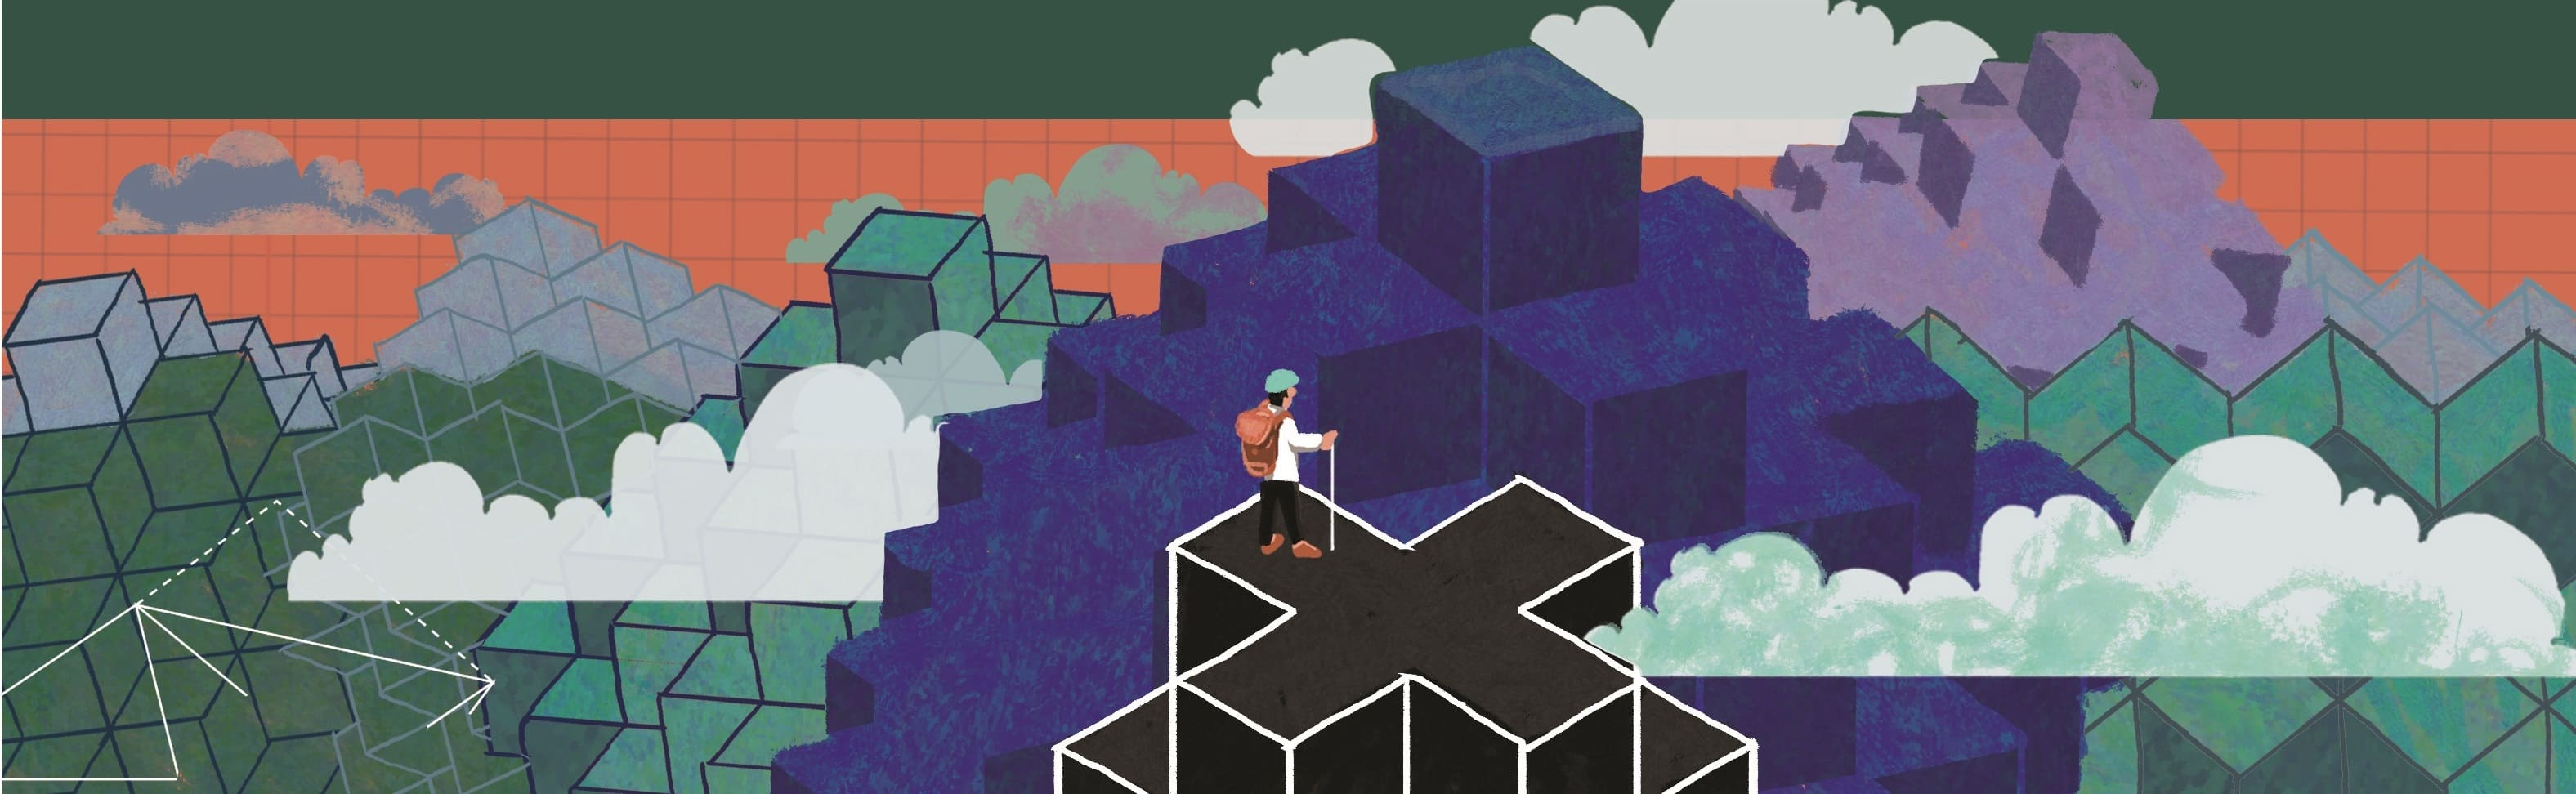
\includegraphics[width=19.3cm]{../thachthuctoanhoc/bannerthachthuc}}}
\centering
\vspace*{4cm}
\endgroup
\vspace*{-8pt}
\begin{tBox}
	\begin{itemize}[leftmargin = 13pt, itemsep = 1.0pt] 
		\item Mỗi bài toán đề xuất (kèm theo lời giải) cần được nêu rõ là bài sáng tác hay bài sưu tầm.
		%		\item Mỗi bài toán đề xuất (kèm theo lời giải) cần được nêu rõ là bài sáng tác hay bài sưu tầm (nếu là bài sưu tầm, cần ghi rõ nguồn).
		\item Bài giải cho mỗi bài toán cần được trình bày trong một file riêng hoặc
		một tờ giấy riêng.
		\item  Người đề xuất bài toán hoặc gửi bài giải cho các bài toán trong mục ``Thách thức kỳ này" cần ghi rõ họ, đệm, tên và nơi làm việc/học tập, số điện thoại liên hệ. Nếu là học sinh (hoặc sinh viên) cần ghi rõ là học sinh lớp mấy (hoặc sinh viên năm thứ mấy).
		\item Các bài toán trong mục Thách thức kỳ này hướng tới các độc giả là học sinh phổ thông; được phân chia thành các mức độ $B$, $A$, và được sắp xếp theo độ khó tăng dần, theo đánh giá chủ quan của Ban biên tập. Các bài toán mức độ $B$ không đòi hỏi các kiến thức vượt quá chương trình môn Toán cấp THCS; các bài toán mức độ $A$ không đòi hỏi các kiến thức vượt quá chương trình môn Toán cấp THPT.
		\item Cách thức gửi bài toán đề xuất hoặc lời giải: gửi file thu được bằng cách scan, ảnh chụp (rõ nét) của bản viết tay, hoặc được soạn thảo bằng các phần mềm Latex, Word tới \url{bbt@pi.edu.vn} hoặc gửi qua đường bưu điện tới Tòa soạn (xem địa chỉ tại bìa $2$).
		\item Hạn gửi lời giải cho các bài toán P$671$--P$680$: trước ngày $15/3/2023$.
	\end{itemize}
\end{tBox}
\begin{center}
	\vspace*{-5pt}
	\textbf{\color{thachthuctoanhoc}\color{thachthuctoanhoc}\color{thachthuctoanhoc}THÁCH THỨC KỲ NÀY}
	\vspace*{-5pt}
\end{center}
\begin{multicols}{2}
	\setlength{\abovedisplayskip}{4pt}
	\setlength{\belowdisplayskip}{4pt}
	{\color{thachthuctoanhoc}{\usefont{T5}{qag}{b}{n} P671.}}
	(Mức $B$) Một hình chữ nhật được chia thành $9$ hình chữ nhật con như hình vẽ. Số ghi ở giữa mỗi hình chữ nhật con bằng chu vi của hình chữ nhật ấy. Biết rằng $c$ là một số nguyên và khác với $2,3,4,5$; hãy tìm $a,b,c,d,e$.
	\begin{center} 
		\definecolor{cqcqcq}{rgb}{0.7529411764705882,0.7529411764705882,0.7529411764705882}
		\begin{tikzpicture}[xscale=1.7,thachthuctoanhoc]
			\draw (0,0) grid (3,3);
			\draw (0.5,1.5) node{$2$};
			\draw (1.5,0.5) node{$5$};
			\draw (1.5,2.5) node{$4$};
			\draw (2.5,1.5) node{$2$};
			\draw (0.5,2.5) node{$a$};
			\draw (2.5,2.5) node{$b$};
			\draw (1.5,1.5) node{$c$};
			\draw (0.5,0.5) node{$d$};
			\draw (2.5,0.5) node{$e$};
		\end{tikzpicture}
	\end{center}
	\begin{flushright}
		\textit{Đăng Hải, Hà Nội (st)}
	\end{flushright}
	{\color{thachthuctoanhoc}{\usefont{T5}{qag}{b}{n} P672.}}
	(Mức $B$) Cho $x$ và $y$ là các số nguyên dương phân biệt thoả mãn $2023x^{2023}+999 y^{2023}$ chia hết cho $x+y$. Chứng minh rằng $x+y$ là hợp số. 
	\begin{flushright}
		\textit{Nguyễn Đức Tấn, Tp. Hồ Chí Minh}
	\end{flushright}
	{\color{thachthuctoanhoc}{\usefont{T5}{qag}{b}{n} P673.}}
	(Mức $B$) Chứng minh rằng,
	\begin{align*}
		A=\sqrt[3]{1^3+1}+\sqrt[3]{2^3+1}+\cdots+\sqrt[3]{2023^3+1}
	\end{align*}
	không phải là số nguyên.
	\begin{flushright}
		\textit{Nguyễn Văn Quý, Hà Nội}
	\end{flushright}
	{\color{thachthuctoanhoc}{\usefont{T5}{qag}{b}{n} P674.}}
	(Mức $B$) Mỗi ô của bảng $8\times 8$ được điền số $+1$ hoặc $-1$ sao cho tổng của $4$ số trong mỗi hình vuông con cỡ $2\times2$ đều bằng $2$ hoặc $-2$. Chứng minh rằng bảng phải chứa hai hàng giống nhau.
	\begin{flushright}
		\textit{Nguyễn Tường Thanh, Nghệ An (st)}
	\end{flushright}
	{\color{thachthuctoanhoc}{\usefont{T5}{qag}{b}{n} P675.}}
	(Mức $B$) Cho hình thang $ABCD$ vuông tại $A$ và $D$. Trên tia $AD$ lấy điểm $F$ sao cho $AF\cdot AD=AB\cdot CD$. Gọi $E$ là hình chiếu vuông góc của $A$ trên $BD$. Chứng minh rằng $\angle CEF=90^\circ$. 
	\begin{figure}[H]
		\vspace*{-5pt}
		\centering
		\captionsetup{labelformat= empty, justification=centering}
		\definecolor{sqsqsq}{rgb}{0.12549019607843137,0.12549019607843137,0.12549019607843137}
		\definecolor{ffqqqq}{rgb}{1,0,0}
		\definecolor{qqzzcc}{rgb}{0,0.6,0.8}
		\definecolor{qqqqff}{rgb}{0,0,1}
		\definecolor{qqqqffa}{rgb}{1,1,1}
		\begin{tikzpicture}[scale=0.55,thachthuctoanhoc]
			\draw[color=sqsqsq] (-3,3.317157287525381) -- (-2.717157287525381,3.317157287525381) -- (-2.717157287525381,3.6) -- (-3,3.6) -- cycle; 
			\draw[color=sqsqsq] (-2.7171572875253815,-3.78) -- (-2.7171572875253815,-3.4971572875253814) -- (-3,-3.4971572875253814) -- (-3,-3.78) -- cycle; 
			\draw[color=sqsqsq] (-0.7031626699615052,2.6414283229649644) -- (-0.8393330759027575,2.315149882755081) -- (-0.5130546356928736,2.1789794768138284) -- (-0.3768842297516215,2.5052579170237124) -- cycle; 
			\draw  (-3,3.6)-- (0.08,3.6);
			\draw  (0.08,3.6)-- (2.48,-3.78);
			\draw [color=qqzzcc] (-3,-3.78)-- (0.08,3.6);
			\draw  (-3,-3.78)-- (2.48,-3.78);
			\draw  (-3,3.6)-- (-3,-3.78);
			\draw [color=ffqqqq] (-3,1.3129539295392954)-- (-0.3768842297516215,2.5052579170237124);
			\draw [color=ffqqqq] (-0.3768842297516215,2.5052579170237124)-- (2.48,-3.78);
			\draw [color=qqzzcc] (-3,3.6)-- (-0.3768842297516215,2.5052579170237124);
			\draw [fill=white] (-3,3.6) circle (1.5pt);
			\draw[color=qqqqff] (-3.04,4.11) node {$A$};
			\draw [fill=white] (0.08,3.6) circle (1.5pt);
			\draw[color=qqqqff] (0.08,4.13) node {$B$};
			\draw [fill=white] (2.48,-3.78) circle (1.5pt);
			\draw[color=qqqqff] (2.9,-3.78) node {$C$};
			\draw [fill=white] (-3,-3.78) circle (1.5pt);
			\draw[color=qqqqff] (-3.6,-3.78) node {$D$};
			\draw [fill=white] (-3,1.3129539295392954) circle (1.5pt);
			\draw[color=qqqqff] (-3.36,1.49) node {$F$};
			\draw [fill=white] (-0.3768842297516215,2.5052579170237124) circle (1.5pt);
			\draw[color=qqqqff] (-0.54,2.99) node {$E$};
		\end{tikzpicture}
		\vspace*{-10pt}
	\end{figure}
	\begin{flushright}
		\textit{Bằng Linh, Phú Thọ}
	\end{flushright}
	{\color{thachthuctoanhoc}{\usefont{T5}{qag}{b}{n} P676.}}
	(Mức $B$) Cho $a, b, c$ là các số thực dương. Chứng minh rằng
	\begin{align*}
		&\sqrt{\frac{a}{b+c}}+\sqrt{\frac{b}{c+a}}+\sqrt{\frac{c}{a+b}}\\
		\leq &\sqrt{\frac{a}{b}+\frac{b}{c}+\frac{c}{a}+\frac{3}{2}} .
	\end{align*}
	\begin{flushright}
		\textit{Nguyễn Việt Hùng, Hà Nội}
	\end{flushright}
	{\color{thachthuctoanhoc}{\usefont{T5}{qag}{b}{n} P677.}}
	(Mức $A$) Cho dãy số thực $(u_n)$ xác định bởi 
	\begin{align*}
		u_n=\dfrac{C^n_{2n}-2022}{n^2}\quad\text{với $n=1,2,3,\ldots$}.
	\end{align*}
	$a)$ Chứng minh rằng $(u_n)$ là dãy tăng và không bị chặn trên.
	\vskip 0.05cm
	$b)$ Tìm tất cả các số thực $\alpha$ sao cho giới hạn $\lim \dfrac{n^\alpha. u_n}{4^n}$ tồn tại hữu hạn và khác $0$. 
	\begin{flushright}
		\textit{Lê Phúc Lữ, Tp. Hồ Chí Minh}
	\end{flushright}
	{\color{thachthuctoanhoc}{\usefont{T5}{qag}{b}{n} P678.}}
	(Mức $A$) Trong mặt phẳng, cho hai điểm $I$, $J$ cố định sao cho $IJ=8$.  Gọi $(S)$ là tập hợp các điểm $M$ thoả mãn ít nhất một trong hai đoạn thẳng $MI,MJ$ không vượt quá $7$. Với $A,B,C$ là ba điểm không thẳng hàng thuộc $(S)$, chu vi tam giác $ABC$ lớn nhất là bao nhiêu?
	\begin{flushright}
		\textit{Trần Quốc Luật, Tp. Hồ Chí Minh}
	\end{flushright}
	{\color{thachthuctoanhoc}{\usefont{T5}{qag}{b}{n} P679.}}
	(Mức $A$) Có $100$ quả trứng xếp thành một vòng tròn. Hỏi, nếu bỏ qua quả đầu tiên, theo chiều kim đồng hồ, ta bắt đầu nhặt từ quả thứ hai, sau đó cứ cách một quả lại nhặt cho đến khi hết trứng, thì quả được nhặt sau cùng là quả thứ mấy?
	\begin{flushright}
		\textit{Phạm Triều Dương, Hà Nội (st)}
	\end{flushright}
	{\color{thachthuctoanhoc}{\usefont{T5}{qag}{b}{n} P680.}}
	(Mức $A$) Xác định tất cả các số nguyên $a$ sao cho: với mỗi số nguyên dương $k$, tồn tại số nguyên dương $n_k$ thoả mãn $2^k\mid n_k^{n_k}+a$. 
	\begin{flushright}
		\textit{Nguyễn Văn Thạch, Đăk Nông}
	\end{flushright}
\end{multicols}
\centerline{{\large{\textbf{\color{thachthuctoanhoc}GIẢI BÀI KỲ TRƯỚC}}}}
\vspace*{-5pt}
\begin{multicols}{2}
	\setlength{\abovedisplayskip}{4pt}
	\setlength{\belowdisplayskip}{4pt}
	{\color{thachthuctoanhoc}{\usefont{T5}{qag}{b}{n} P641.}}
	(Mức $B$)
	Tại mỗi đỉnh của một đa giác lồi $18$ cạnh ở hình dưới đây, người ta ghi một số, sao cho số được ghi ở mỗi đỉnh bằng tổng hai số được ghi ở hai đỉnh kề với nó.
	\begin{figure}[H]
		\vspace*{-5pt}
		\centering
		\captionsetup{labelformat= empty, justification=centering}
		\definecolor{ffvvqq}{rgb}{1,0.3333333333333333,0}
		\definecolor{qqqqffa}{rgb}{0,0,1}
		\definecolor{qqzzff}{rgb}{0,0.6,1}
		\begin{tikzpicture}[line cap=round,line join=round,>=triangle 45,x=1cm,y=1cm,scale=0.45, node font= \small]
			\draw (1.401115339869085,5.50644760016908136) node[anchor=north west] {$X$};
			\draw (1.4408759814898973,-0.7306378725360659) node[anchor=north west] {$Y$};
			\draw (-7.8444170535279,2.5008856260029945) node[anchor=north west] {$S$};
			\draw [color=qqzzff] (0.0915547437082469,-1.9784020259611625)--(1.3147607160299626,-0.9781184915188108);
			\draw [color=qqzzff] (1.3147607160299626,-0.9781184915188108)--(2.122081224105652,0.3802016464606015); 
			\draw [color=qqzzff] (2.122081224105652,0.3802016464606015)--(2.4161414998796458,1.932724932666551); 
			\draw [color=qqzzff] (2.4161414998796458,1.932724932666551)--(2.1614735342261406,3.4921941459791768);
			\draw [color=qqzzff] (2.1614735342261406,3.4921941459791768)--(1.38879404230183,4.87051428395859);
			\draw [color=qqzzff] (1.38879404230183,4.87051428395859)--(0.19129957436757605,5.901439596125702);
			\draw [color=qqzzff] (0.19129957436757605,5.901439596125702)--(-1.2865743636076452,6.4606252749959765);
			\draw [color=qqzzff] (-1.2865743636076452,6.4606252749959765)--(-2.866574363607645,6.480625274995977);
			\draw [color=qqzzff] (-2.866574363607645,6.480625274995977)--(-4.358129107315893,5.959027300957139);
			\draw [color=qqzzff] (-4.358129107315893,5.959027300957139)--(-5.581335079637608,4.958743766514788);
			\draw [color=qqzzff] (-5.581335079637608,4.958743766514788)--(-6.388655587713298,3.600423628535374);
			\draw [color=qqzzff] (-6.388655587713298,3.600423628535374)--(-6.682715863487291,2.0479003423294264);
			\draw [color=qqzzff] (-6.682715863487291,2.0479003423294264)--(-6.428047897833785,0.4884311290167975);
			\draw [color=qqzzff] (-6.428047897833785,0.4884311290167975)--(-5.655368405909476,-0.889889008962613);
			\draw [color=qqzzff] (-5.655368405909476,-0.889889008962613)--(-4.457873937975224,-1.9208143211297237);
			\draw [color=qqzzff] (-4.457873937975224,-1.9208143211297237)--(-2.98,-2.48);
			\draw [color=qqzzff] (-2.98,-2.48)--(-1.4,-2.5);
			\draw [color=qqzzff] (-1.4,-2.5)--(0.0915547437082469,-1.9784020259611625);
			\draw [fill=white] (-2.98,-2.48) circle (1.6pt);
			\draw [fill=white] (-1.4,-2.5) circle (1.6pt);
			\draw [fill=white] (0.0915547437082469,-1.9784020259611625) circle (1.6pt);
			\draw [fill=white] (1.3147607160299626,-0.9781184915188108) circle (1.6pt);
			\draw [fill=white] (2.122081224105652,0.3802016464606015) circle (1.6pt);
			\draw [fill=white] (2.4161414998796458,1.932724932666551) circle (1.6pt);
			\draw [fill=white] (2.1614735342261406,3.4921941459791768) circle (1.6pt);
			\draw [fill=white] (1.38879404230183,4.87051428395859) circle (1.6pt);
			\draw [fill=white] (0.19129957436757605,5.901439596125702) circle (1.6pt);
			\draw [fill=white] (-1.2865743636076452,6.4606252749959765) circle (1.6pt);
			\draw [fill=white] (-2.866574363607645,6.480625274995977) circle (1.6pt);
			\draw [fill=white] (-4.358129107315893,5.959027300957139) circle (1.6pt);
			\draw [fill=white] (-5.581335079637608,4.958743766514788) circle (1.6pt);
			\draw [fill=white] (-6.388655587713298,3.600423628535374) circle (1.6pt);
			\draw [fill=white] (-6.682715863487291,2.0479003423294264) circle (1.6pt);
			\draw [fill=white] (-6.428047897833785,0.4884311290167975) circle (1.6pt);
			\draw [fill=white] (-5.655368405909476,-0.889889008962613) circle (1.6pt);
			\draw [fill=white] (-4.457873937975224,-1.9208143211297237) circle (1.6pt);
		\end{tikzpicture}
		\vspace*{-5pt}
	\end{figure}
	Biết rằng, số được ghi ở đỉnh $X$ là $20$, và số được ghi ở đỉnh $Y$ là $22$. Hãy tìm số được ghi ở đỉnh $S$.
	\vskip 0.05cm
	\textbf{\color{thachthuctoanhoc}Lời giải} (\textit{phỏng theo ý giải của bạn Nguyễn Chánh Thiện, lớp $8/14$, trường THCS Lê Quý Đôn, Quận $3$, Tp. Hồ Chí Minh})\textbf{\color{thachthuctoanhoc}.}
	\vskip 0.05cm
	Xuất phát từ đỉnh $S$, theo chiều kim đồng hồ, ký hiệu các số được ghi tại các đỉnh của $18$--giác, lần lượt, bởi  $x_1,  x_2, \ldots, x_{18}$ (xem Hình dưới đây).
	\vskip 0.05cm
	Do $x_8$, $x_{12}$ là các số được ghi tại các đỉnh $X$, $Y$, nên theo giả thiết của bài ra, $x_8 =20$  và  $x_{12} = 22$.
	\begin{figure}[H]
		\centering
		\vspace*{-10pt}
		\captionsetup{labelformat= empty, justification=centering}
		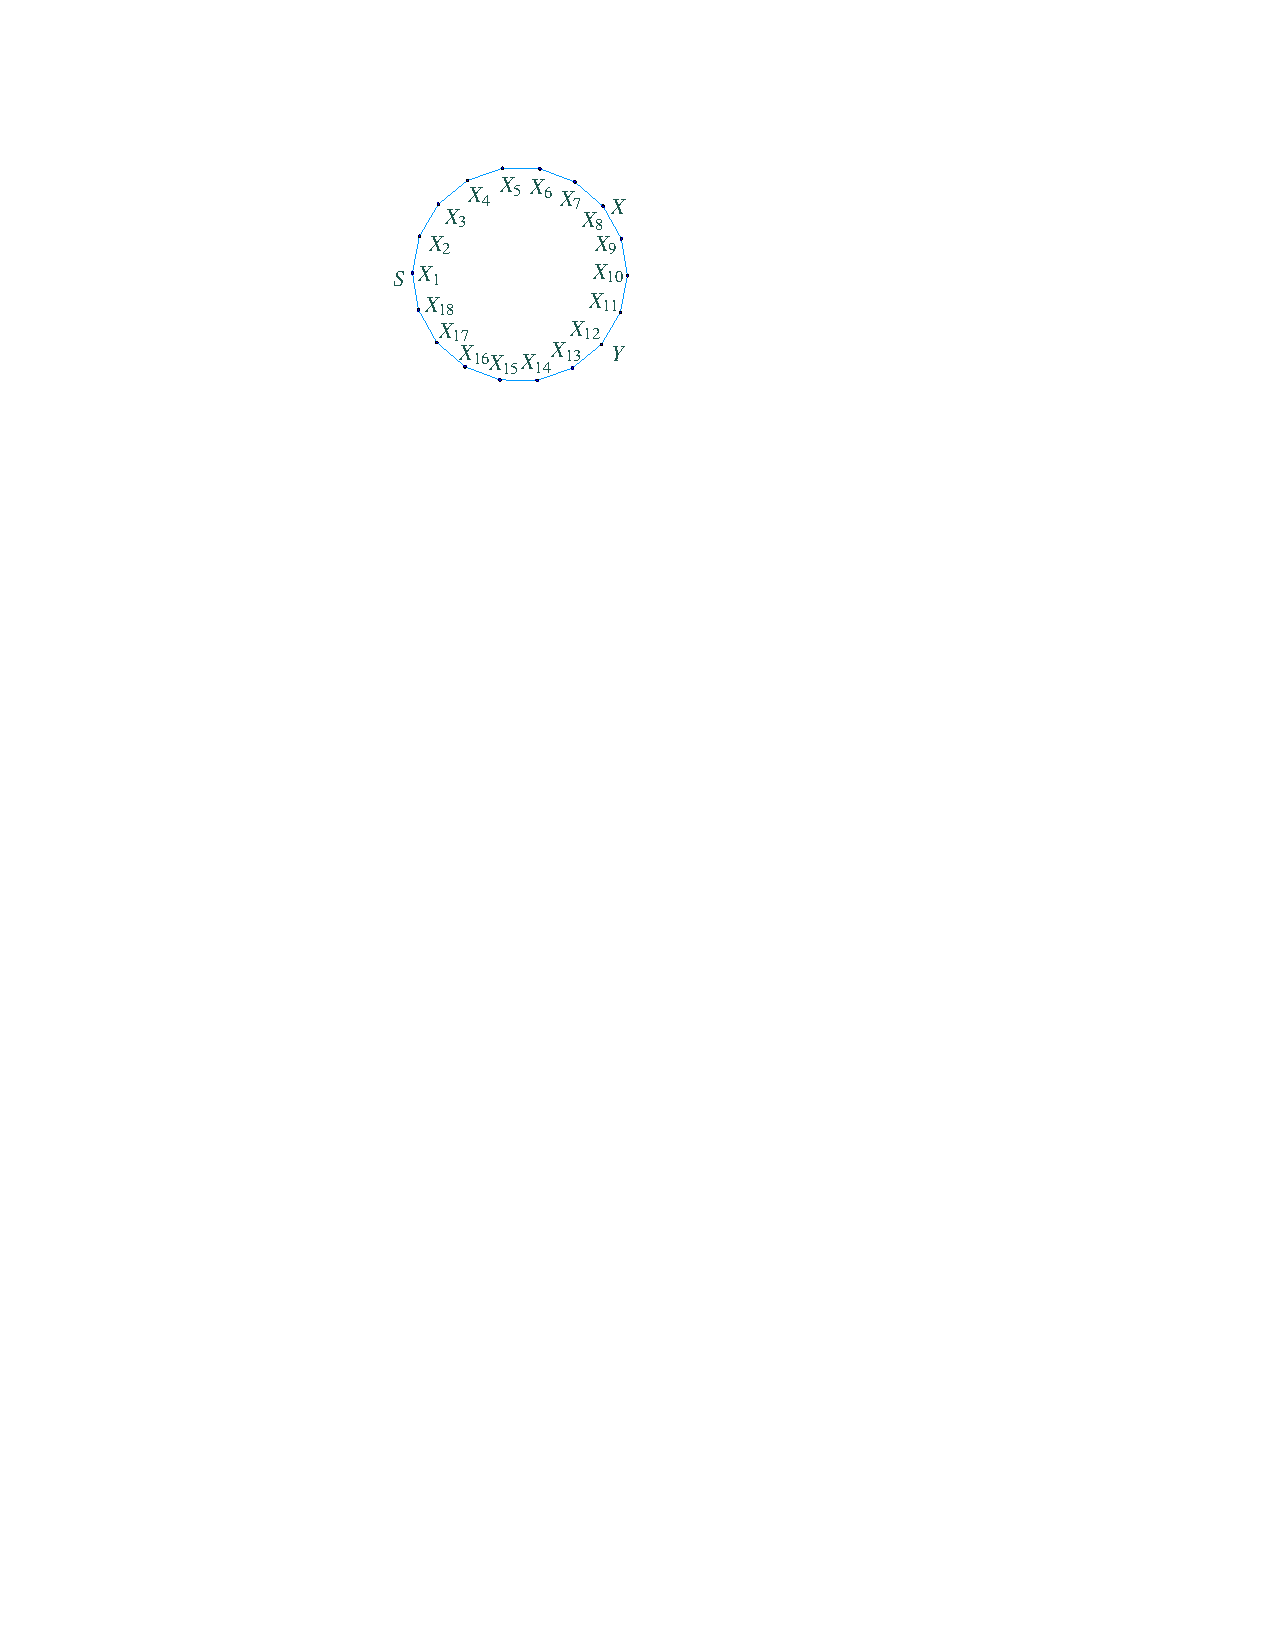
\includegraphics[width=0.75\linewidth]{P641}
		\vspace*{-10pt}
	\end{figure}
	Từ quy tắc ghi số của đề bài suy ra, với mỗi $k = 1, 2, \ldots, 15$, ta có:
	\begin{align*}
		{x_k} &= {x_{k + 1}} - {x_{k + 2}} = {x_{k + 1}} - \left( {{x_{k + 1}} + {x_{k + 3}}} \right) \\
		&=  - {x_{k + 3}}.
	\end{align*}
	Do đó
	\begin{align*}
		&{x_2} =  - {x_5} = {x_8} = 20,\\
		&22 = {x_{12}} =  - {x_{15}} = {x_{18}}.
	\end{align*}
	Vì vậy
	\begin{align*}
		{x_1} = {x_{18}} + {x_2} = 22 + 20 = 42.
	\end{align*}
	Vậy, số được ghi ở đỉnh $S$ là $42$.
	\vskip 0.05cm
	\textbf{\color{thachthuctoanhoc}Bình luận và Nhận xét}
	\vskip 0.05cm	
	Tạp chí đã nhận được nhiều lời giải cho bài toán, từ bạn đọc; và tất cả những lời giải này đều là lời giải đúng.
	\vskip 0.1cm
	\hfill	\textbf{\color{thachthuctoanhoc}Lê Huy}
	\vskip 0.1cm
	{\color{thachthuctoanhoc}{\usefont{T5}{qag}{b}{n} P642.}}
	(Mức $B$)
	Cho $x$, $y$ là các số nguyên dương thỏa mãn $y^2 \!+\! x \!-\! 1$ chia hết cho $xy \!+\! 1$. Chứng minh rằng, tồn tại số tự nhiên $z$, sao cho $x + y + z + xyz$ là một số chính phương.
	\vskip 0.05cm
	\textbf{\color{thachthuctoanhoc}Lời giải} (\textit{của người đề xuất bài toán})\textbf{\color{thachthuctoanhoc}.}
	\vskip 0.05cm
	Từ giả thiết của bài toán, suy ra
	\begin{align*}
		&{xy + 1} \mid x\left( {{y^2} + x - 1} \right) \\
		= &y\left( {xy + 1} \right) + \left( {{x^2} - \left( {x + y} \right)} \right).
	\end{align*}
	Do đó
	\begin{align*}
		{xy + 1} \mid {x^2} - \left( {x + y} \right).
	\end{align*}
	Vì thế, tồn tại số nguyên $z$, sao cho
	\begin{align*}
		{x^2} - \left( {x + y} \right) = z\left( {xy + 1} \right);
	\end{align*}
	hay, $x + y + z + xyz = {x^2}.$
	\vskip 0.05cm  
	Nhận thấy, nếu $z \le -1$  thì
	\begin{align*}
		{x^2} &= x + y + z + xyz \le x + y - 1 - xy \\
		&= - \left( {x - 1} \right)\left( {y - 1} \right) \le 0,
	\end{align*}
	là điều vô lý (do  $x \in \mathbb{N^*}$).
	\vskip 0.05cm
	Vì vậy, $z \ge 0$; hay, $z$ là số tự nhiên.
	\vskip 0.05cm
	Vậy, tồn tại số tự nhiên $z$, sao cho 
	\begin{align*}
		x + y + z + xyz
	\end{align*} là một số chính phương.
	\vskip 0.05cm
	\textbf{\color{thachthuctoanhoc}Bình luận và Nhận xét}
	\vskip 0.05cm
	$\pmb{1.}$ Tác giả bài toán đã chứng minh được rằng, nếu $z_0$  là một số tự nhiên, sao cho $x + y + z_0 + xyz_0$  là một số chính phương, thì tất cả các số tự nhiên $z_k, k \in \mathbb{N^*}$, xác định bởi
	\begin{align*}
		{z_k} = {z_0} + 2xk + \left( {xy + 1} \right){k^2},
	\end{align*}
	cũng có tính chất như vậy. Vì thế, kết luận của bài ra có thể được mở rộng thành: “Có vô số số tự nhiên $z$, sao cho $x + y + z + xyz$ là một số chính phương.”
	\vskip 0.05cm
	$\pmb{2.}$ Theo ý giải của bạn \textit{Vương Khánh Toàn} (lớp $10$A$1$ Toán, trường THPT chuyên KHTN, trường ĐHKHTN, ĐHQG Hà Nội), có thể chứng minh được rằng, các số nguyên dương $x$, $y$ thỏa mãn điều kiện của bài ra khi và chỉ khi $x = k + 1, y = k(k + 1)$, trong đó, $k$ là một số nguyên dương tùy ý. Từ đây, dễ thấy, chọn $z = 0$, ta sẽ có số tự nhiên $z$ thỏa mãn yêu cầu đề bài.
	\vskip 0.05cm
	$\pmb{3.}$ Rất tiếc, trong số các lời giải Tạp chí đã nhận được từ bạn đọc, có một số lời giải sai, do người giải bài đã mắc một trong các lỗi sau đây:
	\vskip 0.05cm
	-- \textit{Ngộ nhận} rằng, không mất tính tổng quát, có thể giả sử $x^2 > x + y$;
	\vskip 0.05cm 
	-- \textit{Hiểu sai} rằng, số nguyên $a$ chia hết cho số nguyên $b$ khi và chỉ khi tồn tại số \textit{tự nhiên} $q$, sao cho $a = bq$;
	\vskip 0.05cm
	--\textit{ Suy luận sai} rằng, với $x$, $y$ là các số nguyên dương, và $a$ là số nguyên âm, từ
	\begin{align*}
		{x^2} - x - y = a\left( {xy + 1} \right)
	\end{align*}
	suy ra, $x^2 - x - y = 0$.
	\vskip 0.05cm  
	Cùng với các lời giải sai nêu trên, có một lời giải không được coi là lời giải hoàn chỉnh, do các lập luận thiếu chặt chẽ, thiếu chính xác.
	\begin{flushright}
		\textbf{\color{thachthuctoanhoc}Lưu Thị Thanh Hà}
	\end{flushright}
	{\color{thachthuctoanhoc}{\usefont{T5}{qag}{b}{n} P643.}}
	(Mức $B$)
	Người ta lần lượt ghi các số lên bảng, theo quy tắc: Ở mỗi lần ghi, chỉ ghi một số, và nếu số được ghi ở lần thứ $k$ ($k \in \mathbb{N^*}$) là $x \ne -1$,  thì ở lần thứ $k + 1$ ghi số $\dfrac{x-1}{x+1}$. Hãy tìm số nhỏ nhất cần ghi ở lần thứ nhất, sao cho trong quá trình ghi số lên bảng theo quy tắc trên, ta ghi được số $-\dfrac{1}{2023}$.
	\vskip 0.05cm
	\textbf{\color{thachthuctoanhoc}Lời giải} (\textit{của người chấm bài})\textbf{\color{thachthuctoanhoc}.}
	\vskip 0.05cm
	Với mỗi $k \in \mathbb{N^*}$,  ký hiệu $x_k$  là số được ghi lên bảng ở lần ghi thứ $k$.
	\vskip 0.05cm
	Gọi $a$ là số được ghi lên bảng ở lần ghi đầu tiên; ta có $x_1 = a$.
	\vskip 0.05cm 
	Theo quy tắc ghi số của bài ra, để có thể ghi tiếp một số mới lên bảng, cần có $a \ne -1$.  Khi đó, ta có
	\begin{align*}
		{x_2} = \frac{{a - 1}}{{a + 1}}.
	\end{align*}
	Dễ thấy, $x_2 \ne -1$   khi và chỉ khi $a \ne 0$. Do đó, với $a \ne 0 ,-1$,   ta có
	\begin{align*}
		{x_3} = \frac{{{x_2} - 1}}{{{x_2} + 1}} =  - \frac{1}{a}.
	\end{align*}
	Vì $x_3 \ne -1$ khi và chỉ khi $a \ne 1$, nên với $a \ne 0, \pm 1$  ta có:
	\begin{align*}
		{x_4} = \frac{{{x_3} - 1}}{{{x_3} + 1}} =  - \frac{{a + 1}}{{a - 1}}.
	\end{align*}
	Do $x_4 \ne -1$ với mọi $a$, nên
	\begin{align*}
		{x_5} = \frac{{{x_4} - 1}}{{{x_4} + 1}} = a = {x_1}.
	\end{align*}
	Từ những điều nêu trên, suy ra:
	\vskip 0.05cm
	-- Nếu $a = -1$  thì ta ghi được lên bảng duy nhất số $-1$.
	\vskip 0.05cm 
	-- Nếu $a = 0$ thì ta ghi được lên bảng hai số, là $0$ và $-1$.
	\vskip 0.05cm 
	-- Nếu $a = 1$ thì ta ghi được lên bảng ba số, là $1$, $0$ và $-1$.
	\vskip 0.05cm 
	-- Nếu $a\ne 0, \pm 1$,  thì tất cả các số ghi được lên bảng là $a, \dfrac{a-1}{a+1}, -\dfrac{1}{a}, -\dfrac{a+1}{a-1}$.
	\vskip 0.05cm      
	Vì vậy, ta ghi được lên bảng số $-\dfrac{1}{2023}$  khi và chỉ khi $a \ne 0, \pm 1$, và đồng thời, một trong bốn số vừa nêu trên bằng $-\dfrac{1}{2023}$.
	\vskip 0.05cm
	Ta có:
	\begin{align*}
		\frac{{a - 1}}{{a + 1}} =  - \frac{1}{{2023}}& \Leftrightarrow a = \frac{1011}{1012};\\
		-\dfrac{1}{a} = - \frac{1}{2023} &\Leftrightarrow a = 2023;\\
		-\dfrac{a +1}{a-1} = -\dfrac{1}{2023} &\Leftrightarrow a = - \dfrac{1012}{1011}.
	\end{align*}
	Do đó, ta ghi được lên bảng số $-\dfrac{1}{2023}$  khi và chỉ khi $a \in \left\{ { - \dfrac{1}{{2023}};\dfrac{{1011}}{{1012}};2023; - \dfrac{{1012}}{{1011}}} \right\}$.   Dễ thấy,  $-\dfrac{1012}{1011}$ là số nhỏ nhất trong bốn số thuộc tập hợp vừa nêu. Vì vậy, số nhỏ nhất cần ghi ở lần đầu tiên, sao cho có thể ghi lên bảng số  $-\dfrac{1}{2023}$, là  $-\dfrac{1012}{1011}$.
	\vskip 0.1cm
	\textbf{\color{thachthuctoanhoc}Bình luận và Nhận xét}
	\vskip 0.1cm
	$\pmb{1.}$ Xét về logic, trong quy tắc ghi số của bài ra, cần nêu rõ, nếu số được ghi lên bảng là $-1$ thì việc ghi số sẽ tiếp tục thế nào? Dừng lại, không ghi số nữa, hay ghi tiếp số nào? Lời giải trên đây là lời giải dựa trên việc hiểu quy tắc ghi số của bài ra, theo hướng: Việc ghi số lên bảng sẽ dừng lại, ngay sau khi số được ghi là $-1$.
	\vskip 0.05cm
	$\pmb{2.}$ Rất tiếc, tất cả các lời giải Tạp chí nhận được từ bạn đọc đều không được coi là lời giải hoàn chỉnh, do người giải bài đã khẳng định \textit{không đúng} rằng, với $a$ (theo ký hiệu trong Lời giải trên) là số tùy ý, các số ghi được lên bảng \textit{luôn là} $a, \dfrac{a-1}{a+1}, - \dfrac{1}{a}, - \dfrac{a+1}{a-1}$.      
	\begin{flushright}
		\textbf{\color{thachthuctoanhoc}Hà Thanh}
	\end{flushright}
	{\color{thachthuctoanhoc}{\usefont{T5}{qag}{b}{n} P644.}}
	(Mức $B$)
	Xét tam giác $ABC$ có các góc $B$, $C$ nhọn. Gọi $H$ là chân đường cao kẻ từ $A$ của tam giác đó. Chứng minh rằng $ABC$ là tam giác vuông tại $A$ khi và chỉ khi
	\begin{align*}
		\frac{{H{B^3}}}{{A{B^4}}} + \frac{{H{C^3}}}{{A{C^4}}} = \frac{1}{{BC}}.
	\end{align*}
	\textbf{\color{thachthuctoanhoc}Lời giải} (\textit{dựa theo lời giải của bạn Vũ Bảo Lân, lớp $8$A$5$, trường THCS Phúc Yên, Tp. Phúc Yên, tỉnh Vĩnh Phúc})\textbf{\color{thachthuctoanhoc}.}
	\vskip 0.05cm
	$\pmb{1.}$ \textit{Chứng minh “chỉ khi”.
		\vskip 0.05cm
		Giả sử tam giác $ABC$ vuông tại} $A$ (xem Hình $1$) .\textit{Ta cần chứng minh}
	\begin{align*}
		\frac{{H{B^3}}}{{A{B^4}}} + \frac{{H{C^3}}}{{A{C^4}}} = \frac{1}{{BC}}. \tag{$1$}
	\end{align*}                                                           
	\begin{figure}[H]
		\centering
		\vspace*{-5pt}
		\captionsetup{labelformat= empty, justification=centering}
		\begin{tikzpicture}[scale=0.6,thachthuctoanhoc]
			\draw[] (2.8557926412572288,2.657631836505606) -- (3.07873080533295,2.4835669779081666) -- (3.2527956639303897,2.7065051419838877) -- (3.029857499854668,2.8805700005813275) -- cycle; 
			\draw[] (3.312700212329287,-1.) -- (3.312700212329287,-0.7171572875253811) -- (3.029857499854668,-0.7171572875253811) -- (3.029857499854668,-1.) -- cycle; 
			\draw [] (0.,-1.)-- (8.,-1.);
			\draw [] (3.029857499854668,2.8805700005813275)-- (0.,-1.);
			\draw [] (3.029857499854668,2.8805700005813275)-- (8.,-1.);
			\draw [] (3.029857499854668,-1.)-- (3.029857499854668,2.8805700005813275);
			\draw (2.78,3.85) node[anchor=north west] {$A$};
			\draw (-0.48,-0.95) node[anchor=north west] {$B$};
			\draw (7.85,-0.95) node[anchor=north west] {$C$};
			\draw (2.72,-0.95) node[anchor=north west] {$H$};
			\draw [fill=white] (0.,-1.) circle (1.5pt);
			\draw [fill=white] (8.,-1.) circle (1.5pt);
			\draw [fill=white] (3.029857499854668,2.8805700005813275) circle (1.5pt);
			\draw [fill=white] (3.029857499854668,-1.) circle (1.5pt);
		\end{tikzpicture}
		\caption{\small\textit{\color{thachthuctoanhoc}Hình $1$.}}
		\vspace*{-10pt}
	\end{figure}
	Do $H$ là chân đường cao kẻ từ đỉnh góc vuông của tam giác vuông $ABC$ nên
	\begin{align*}
		A{B^2} = &BC \cdot BH, \,\,\,AC^2 = BC \cdot CH,\\
		&\text{và }	BC = HB + HC.
	\end{align*}
	Do đó
	\begin{align*}
		\frac{{H{B^3}}}{{A{B^4}}} + \frac{{H{C^3}}}{{A{C^4}}} &= \frac{{H{B^3}}}{{B{C^2} \cdot H{B^2}}} + \frac{{H{C^3}}}{{B{C^2} \cdot H{C^2}}} \\
		&= \frac{{HB + HC}}{{B{C^2}}} = \frac{1}{{BC}}.
	\end{align*}
	($1$) được chứng minh.
	\vskip 0.05cm
	$\pmb{2.}$ \textit{Chứng minh “khi”.
		\vskip 0.05cm
		Giả sử $ABC$ là tam giác thỏa mãn ($1$), và có các góc $B$, $C$ là góc nhọn. 
		Ta cần chứng minh tam giác $ABC$ vuông tại $A$.}
	Gọi $A'$ là giao điểm của tia $HA$ và đường tròn đường kính $BC$; ta có $\angle BA'C = 90^\circ$,  và $H$ là chân đường cao kẻ từ $A'$  của tam giác vuông $A'BC$. Do đó, theo chứng minh ở phần $1$, ta có:
	\begin{align*}
		\frac{{H{B^3}}}{{A'{B^4}}} + \frac{{H{C^3}}}{{A'{C^4}}} = \frac{1}{{BC}}. \tag{$2$}	
	\end{align*}
	Nhận thấy:
	\vskip 0.05cm
	-- Nếu góc $A$ là góc nhọn (xem Hình $2$) thì điểm $A$ nằm bên ngoài đường tròn đường kính $BC$.
	\begin{figure}[H]
		\centering
		%		\vspace*{-5pt}
		\captionsetup{labelformat= empty, justification=centering}
		\begin{tikzpicture}[scale=0.6,thachthuctoanhoc]
			\draw[] (2.,0.28284271247461906) -- (1.7171572875253809,0.28284271247461906) -- (1.7171572875253809,0.) -- (2.,0.) -- cycle; 
			\draw[] (1.8267949192431123,3.6493765484574374) -- (2.0504017169930915,3.4761714677005497) -- (2.223606797749979,3.699778265450529) -- (2.,3.8729833462074166) -- cycle; 
			\draw [] (-1.,0.)-- (7.,0.);
			\draw [] (2.,3.8729833462074166)-- (-1.,0.);
			\draw [] (2.,3.8729833462074166)-- (7.,0.);
			\draw [] (2.,6.)-- (-1.,0.);
			\draw [] (2.,6.)-- (7.,0.);
			\draw [] (2.,0.)-- (2.,6.);
			\draw [shift={(3.,0.)},]  plot[domain=0.:3.141592653589793,variable=\t]({1.*4.*cos(\t r)+0.*4.*sin(\t r)},{0.*4.*cos(\t r)+1.*4.*sin(\t r)});
			\draw (1.9,6.74) node[anchor=north west] {$A$};
			\draw (-1.46,0) node[anchor=north west] {$B$};
			\draw (6.75,0) node[anchor=north west] {$C$};
			\draw (1.85,0) node[anchor=north west] {$H$};
			\draw (1.8,4.95) node[anchor=north west] {$A'$};
			\draw [fill=white] (-1.,0.) circle (1.5pt);
			\draw [fill=white] (7.,0.) circle (1.5pt);
			\draw [fill=white] (3.,0.) circle (1.5pt);
			\draw [fill=white] (2.,0.) circle (1.5pt);
			\draw [fill=white] (2.,3.8729833462074166) circle (1.5pt);
			\draw [fill=white] (2.,6.) circle (1.5pt);
		\end{tikzpicture}
		\caption{\small\textit{\color{thachthuctoanhoc}Hình $2$.}}
		\vspace*{-10pt}
	\end{figure}
	Vì thế, điểm $A'$ nằm giữa hai điểm $H$, $A$. Suy ra, $AB > A'B$  và $AC > A'C$.  Do đó, với lưu ý tới ($2$), ta có:
	\begin{align*}
		\frac{{H{B^3}}}{{A{B^4}}} + \frac{{H{C^3}}}{{A{C^4}}} < \frac{{H{B^3}}}{{A'{B^4}}} + \frac{{H{C^3}}}{{A'{C^4}}} = \frac{1}{{BC}},
	\end{align*}
	mâu thuẫn với ($1$). Vì vậy, góc $A$ không thể là góc nhọn.                     \hfill ($3$)
	\vskip 0.05cm
	-- Nếu góc $A$ là góc tù (xem Hình $3$) thì điểm $A$ nằm bên trong đường tròn đường kính $BC$.
	\begin{figure}[H]
		\centering
		\vspace*{-5pt}
		\captionsetup{labelformat= empty, justification=centering}
		\begin{tikzpicture}[scale=0.6,thachthuctoanhoc]
			\draw[] (1.8267949192431123,4.649376548457438) -- (2.0504017169930915,4.47617146770055) -- (2.223606797749979,4.699778265450529) -- (2.,4.872983346207417) -- cycle; 
			\draw[] (2.,1.2828427124746191) -- (1.7171572875253809,1.2828427124746191) -- (1.7171572875253809,1.) -- (2.,1.) -- cycle; 
			\draw [] (-1.,1.)-- (7.,1.);
			\draw [] (2.,3.)-- (-1.,1.);
			\draw [] (2.,3.)-- (7.,1.);
			\draw [shift={(3.,1.)},]  plot[domain=0.:3.141592653589793,variable=\t]({1.*4.*cos(\t r)+0.*4.*sin(\t r)},{0.*4.*cos(\t r)+1.*4.*sin(\t r)});
			\draw [] (2.,4.872983346207417)-- (-1.,1.);
			\draw [] (2.,4.872983346207417)-- (7.,1.);
			\draw [] (2.,1.)-- (2.,4.872983346207417);
			\draw (1.76,6) node[anchor=north west] {$A'$};
			\draw (1.8,3.85) node[anchor=north west] {$A$};
			\draw (-1.44,0.85) node[anchor=north west] {$B$};
			\draw (1.74,0.85) node[anchor=north west] {$H$};
			\draw (6.75,0.85) node[anchor=north west] {$C$};
			\draw [fill=white] (-1.,1.) circle (1.5pt);
			\draw [fill=white] (7.,1.) circle (1.5pt);
			\draw [fill=white] (3.,1.) circle (1.5pt);
			\draw [fill=white] (2.,1.) circle (1.5pt);
			\draw [fill=white] (2.,4.872983346207417) circle (1.5pt);
			\draw [fill=white] (2.,3.) circle (1.5pt);
		\end{tikzpicture}
		\caption{\small\textit{\color{thachthuctoanhoc}Hình $3$.}}
		\vspace*{-10pt}
	\end{figure}
	Vì thế, điểm $A$ nằm giữa hai điểm $H, A'$. Suy ra, $AB < A'B$ và $AC < A'C$.  Do đó, với lưu ý tới ($2$), ta có:
	\begin{align*}
		\frac{{H{B^3}}}{{A{B^4}}} + \frac{{H{C^3}}}{{A{C^4}}} > \frac{{H{B^3}}}{{A'{B^4}}} + \frac{{H{C^3}}}{{A'{C^4}}} = \frac{1}{{BC}},
	\end{align*}
	mâu thuẫn với ($1$). Vì vậy, góc $A$ không thể là góc tù.  \hfill ($4$)
	\vskip 0.05cm
	Từ ($3$) và ($4$) suy ra, góc $A$ là góc vuông; và do đó, ta có điều cần chứng minh.
	\vskip 0.05cm
	\textbf{\color{thachthuctoanhoc}Bình luận và Nhận xét}
	\vskip 0.05cm
	Rất tiếc, trong số các lời giải Tạp chí đã nhận được từ bạn đọc, có một số lời giải sai, do người giải bài đã mắc một trong các lỗi sau:
	\vskip 0.05cm
	-- \textit{Mới chỉ chứng minh được}, nếu tam giác $ABC$ vuông tại $A$ thì ta có hệ thức đã nêu trong đề bài;
	\vskip 0.05cm
	-- \textit{Ngộ nhận} rằng, hiển nhiên có
	\begin{align*}
		&HB\!\left(\!\!\!\frac{{H{B^2}}}{{A{B^4}}} \!-\! \frac{1}{{B{C^2}}}\!\!\! \right)\!\!+\! HC \! \left(\!\!\!\frac{{H{C^2}}}{{A{C^4}}} \!-\! \frac{1}{{B{C^2}}} \!\!\!\right) \!\!=\! 0\\
		\Leftrightarrow &\frac{{H{B^2}}}{{A{B^4}}} - \frac{1}{{B{C^2}}} = \frac{{H{C^2}}}{{A{C^4}}} - \frac{1}{{B{C^2}}} = 0.
	\end{align*}
	\begin{flushright}
		\textbf{\color{thachthuctoanhoc}Hạ Vũ Anh}
	\end{flushright}
	{\color{thachthuctoanhoc}{\usefont{T5}{qag}{b}{n} P645.}}
	(Mức $B$)
	Cho $a$, $b$, $c$ là các số thực dương thỏa mãn $abc = 1$. Chứng minh rằng
	\begin{align*}
		&\frac{a}{{a + {b^3}c + b}} + \frac{b}{{b + {c^3}a + c}} \\
		&+ \frac{c}{{c + {a^3}b + a}} \ge 1.
	\end{align*}
	\textbf{\color{thachthuctoanhoc}Lời giải} (\textit{dựa theo lời giải của người đề xuất bài toán})\textbf{\color{thachthuctoanhoc}.}
	\vskip 0.05cm
	Do $abc = 1$ nên
	\begin{align*}
		\frac{a}{{a \!+\! {b^3}c \!+\! b}} \!=\! \frac{{{a^2}}}{{{a^2} \!+\! a{b^3}c \!+\! ab}} \!=\! \frac{{{a^2}}}{{{a^2} \!+\! ab \!+\! {b^2}}}.
	\end{align*}
	Bằng cách hoàn toàn tương tự, ta có:
	\begin{align*}
		&\frac{b}{{b + {c^3}a + c}} = \frac{{{b^2}}}{{{b^2} + bc + {c^2}}},\\ &\frac{c}{{c + {a^3}b + a}} = \frac{{{c^2}}}{{{c^2} + ca + {a^2}}}.
	\end{align*}
	Do đó, bất đẳng thức cần chứng minh của đề bài tương đương với bất đẳng thức
	\begin{align*}
		&\frac{{{a^2}}}{{{a^2} + ab + {b^2}}} + \frac{{{b^2}}}{{{b^2} + bc + {c^2}}} \\
		&+ \frac{{{c^2}}}{{{c^2} + ca + {a^2}}} \ge 1. \tag{$1$}
	\end{align*}
	Theo bất đẳng thức Cauchy -- Schwarz cho hai số thực dương, ta có:
	\begin{align*}
		&\frac{{{a^2}}}{{{a^2} + ab + {b^2}}} + \frac{c}{{a + b + c}} \\
		= &\frac{{{a^2}}}{{{a^2} + ab + {b^2}}} + \frac{{{c^2}}}{{ac + bc + {c^2}}} \\
		\ge &\frac{{{{\left( {a + c} \right)}^2}}}{{{a^2} + {b^2} + {c^2} + ab + bc + ca}}. \tag{$2$}
	\end{align*}
	Bằng cách hoàn toàn tương tự, ta cũng chứng minh được:
	\begin{align*}
		&\frac{{{b^2}}}{{{b^2} + bc + {c^2}}} + \frac{a}{{a + b + c}} \\
		\ge &\frac{{{{\left( {b + a} \right)}^2}}}{{{a^2} + {b^2} + {c^2} + ab + bc + ca}} \tag{$3$}\\
		&\frac{{{c^2}}}{{{c^2} + ca + {a^2}}} + \frac{b}{{a + b + c}} \\
		\ge &\frac{{{{\left( {c + b} \right)}^2}}}{{{a^2} + {b^2} + {c^2} + ab + bc + ca}}. \tag{$4$}
	\end{align*}
	Cộng các bất đẳng thức ($2$), ($3$), ($4$), vế theo vế, ta được:
	\begin{align*}
		&\frac{{{a^2}}}{{{a^2}+ ab + {b^2}}} + \frac{{{b^2}}}{{{b^2} + bc + {c^2}}} \\
		&+ \frac{{{c^2}}}{{{c^2} + ca + {a^2}}} + 1\\[+1ex]
		\ge &\frac{{{{\left( {a + c} \right)}^2} + {{\left( {b + a} \right)}^2} + {{\left( {c + b} \right)}^2}}}{{{a^2} + {b^2} + {c^2} + ab + bc + ca}}\\[+1ex]
		= &\frac{{2\left( {{a^2} + {b^2} + {c^2} + ab + bc + ca} \right)}}{{{a^2} + {b^2} + {c^2} + ab + bc + ca}} = 2.
	\end{align*}
	Suy ra
	\begin{align*}
		&\frac{{{a^2}}}{{{a^2} + ab + {b^2}}} + \frac{{{b^2}}}{{{b^2} + bc + {c^2}}} \\
		&+ \frac{{{c^2}}}{{{c^2} + ca + {a^2}}} \ge 1.
	\end{align*}
	Bất đẳng thức ($1$) được chứng minh; và do đó, bất đẳng thức của đề bài được chứng minh.
	\vskip 0.05cm
	\textbf{\color{thachthuctoanhoc}Bình luận và Nhận xét}
	\vskip 0.05cm
	$\pmb{1.}$ Từ Lời giải trên dễ thấy, bất đẳng thức của bài ra là một biến thể đơn sơ, nhẹ nhàng của bất đẳng thức ($1$).
	\vskip 0.05cm
	$\pmb{2.}$ Bất đẳng thức ($1$) là một bất đẳng thức đã có từ lâu. Tác giả Vasile Cirtoaje đã giới thiệu bất đẳng thức này trong cuốn sách “\textit{Algebraic Inequalities: Old and New Method}” (bài số $10$, trang $21$), do Nhà xuất bản GIL phát hành năm $2006$. Trong cuốn sách này, Vasile Cirtoaje đã giới thiệu một cách chứng minh rất độc đáo cho bất đẳng thức đó,  như sau:
	\vskip 0.05cm
	“Đặt $x = {a^2} + ab + {b^2},$ $y = {b^2} + bc + {c^2},$      và $z = {c^2} + ca + {a^2}$.  Ta có:
	\begin{align*}
		&\left( {\frac{1}{x} + \frac{1}{y} + \frac{1}{z}} \right)\left( {\frac{{{a^2}}}{x} + \frac{{{b^2}}}{y} + \frac{{{c^2}}}{z}} \right)\\
		= &\frac{{{a^2}}}{{{x^2}}} \!+\! \frac{{{b^2}}}{{{y^2}}} \!+\! \frac{{{c^2}}}{{{z^2}}} \!+\! \frac{{{a^2} \!+\! {b^2}}}{{xy}} \!+\! \frac{{{b^2} \!+\! {c^2}}}{{yz}} \!+\! \frac{{{c^2} \!+\! {a^2}}}{{zx}}\\
		\ge &\frac{{ab}}{{xy}} \!+\! \frac{{bc}}{{yz}} \!+\! \frac{{ca}}{{zx}} \!+\! \frac{{{a^2} \!+\! {b^2}}}{{xy}} \!+\! \frac{{{b^2} \!+\! {c^2}}}{{yz}} \!+\! \frac{{{c^2}\! +\! {a^2}}}{{zx}}\\
		= &\frac{1}{y} + \frac{1}{z} + \frac{1}{x}.
	\end{align*}
	Từ đó, hiển nhiên thu được bất đẳng thức ($1$).”
	\vskip 0.05cm
	$\pmb{3.}$ Rất tiếc, trong số các lời giải Tạp chí đã nhận được từ bạn đọc, có hai lời giải sai, do người giải bài đã mắc một trong các lỗi sau:
	\vskip 0.05cm
	-- \textit{Thực hiện sai một số biến đổi}; chẳng hạn:
	\begin{align*}
		\frac{{{a^2}}}{{{a^2} + ab + {b^2}}} = {a^2}\left( {1 - \frac{{ab + {b^2}}}{{{a^2} + ab + {b^2}}}} \right).
	\end{align*}
	-- \textit{Nhầm chiều bất đẳng thức}; chẳng hạn:
	\begin{align*}
		&\frac{{{{\left( {a + b + c} \right)}^2}}}{{{{\left( {a \!+\! b \!+\! c} \right)}^2} \!+\! \left( {{a^2} \!+\! {b^2} \!+\! {c^2} \!-\! ab \!-\! bc \!-\! ca} \right)}} \\
		\ge &\frac{{{{\left( {a + b + c} \right)}^2}}}{{{{\left( {a + b + c} \right)}^2}}}.
	\end{align*}
	\begin{flushright}
		\textbf{\color{thachthuctoanhoc}Võ Quốc Bá Cẩn}
	\end{flushright}
	{\color{thachthuctoanhoc}{\usefont{T5}{qag}{b}{n} P646.}}
	(Mức $B$)
	Chứng minh rằng, trong mỗi bát giác lồi, luôn có ít nhất ba đường chéo mà độ dài của chúng đôi một khác nhau.
	(Bát giác là một đa giác có $8$ cạnh.)
	\vskip 0.05cm
	\textbf{\color{thachthuctoanhoc}Lời giải} (\textit{của người chấm bài})\textbf{\color{thachthuctoanhoc}.}
	\vskip 0.05cm
	Xét một bát giác lồi tùy ý; gọi là ($H$).
	\vskip 0.05cm
	Do ($H$) là bát giác lồi, nên mỗi đỉnh của nó đều không nằm bên trong bất kỳ tam giác nào có ba đỉnh là ba đỉnh của bát giác đó. Do đó, đường trung trực của mỗi cạnh của ($H$) chỉ có thể đi qua tối đa một đỉnh của nó. \hfill ($1$)
	\vskip 0.05cm
	Cũng do ($H$) là bát giác lồi, nên đường trung trực của mỗi đường chéo của nó không đi qua hai đỉnh kề nhau của bát giác.                 \hfill ($2$)
	\vskip 0.05cm
	Xét một cạnh tùy ý của ($H$); gọi cạnh này là $AB$. Gọi $C$ là đỉnh khác $B$ và kề với $A$; gọi $D$ là đỉnh khác $A$ và kề với $B$.
	\vskip 0.05cm
	Theo ($1$), ngoại trừ bốn đỉnh $C$, $A$, $B$, $D$, trong bốn đỉnh còn lại của ($H$) chỉ có tối đa một đỉnh cách đều $A$ và $B$. Do đó, trong bốn đỉnh đó, tồn tại ba đỉnh, mà mỗi đỉnh đều \textit{không} cách đều $A$ và $B$. Gọi ba đỉnh này là $X$, $Y$, $Z$; ta có $XA \ne XB$, $YA \ne YB$, và $ZA \ne ZB$. Xảy ra một trong các trường hợp sau:
	\vskip 0.05cm
	$\diamond$ \textit{Trường hợp} $1$: $YA \ne XA$ và $YA \ne XB$.
	\vskip 0.05cm
	Trong trường hợp này, $XA$, $XB$, $YA$ là ba đường chéo có độ dài đôi một khác nhau.
	\vskip 0.05cm
	$\diamond$ \textit{Trường hợp} $2$: $YA = XA$.
	\vskip 0.05cm
	Khi đó, $YB \ne XA$ (do $YB \ne YA$), và \linebreak$YB \ne XB$ (vì nếu ngược lại, $YB = XB$, thì đường trung trực của $XY$ đi qua hai đỉnh $A$, $B$, mâu thuẫn với ($1$), hoặc với ($2$), tùy thuộc $XY$ là cạnh, hay là đường chéo, của ($H$)). Do đó, $XA, XB, YB$ là ba đường chéo có độ dài đôi một khác nhau.
	\vskip 0.05cm
	$\diamond$ \textit{Trường hợp} $3$: $YA = XB$.
	\vskip 0.05cm
	Khi đó:
	\vskip 0.05cm
	-- Nếu $ZA \ne XA$ và $ZA \ne XB$ thì $XA, XB, ZA$ là ba đường chéo có độ dài đôi một khác nhau.
	\vskip 0.05cm
	-- Nếu $ZA = XA$ thì bằng các lập luận tương tự như ở trường hợp $2$, ta có $XA$, $XB$, $ZB$ là ba đường chéo có độ dài đôi một khác nhau.
	\vskip 0.05cm
	-- Nếu $ZA = XB$ thì $ZA = YA$ (do $YA = XB$). Do đó, bằng các lập luận tương tự như ở trường hợp $2$, ta có $YA$, $YB$, $ZB$ là ba đường chéo có độ dài đôi một khác nhau.
	\vskip 0.05cm
	Vậy, trong ($H$) có ít nhất ba đường chéo có độ dài đôi một khác nhau.
	\vskip 0.05cm
	Vì ($H$) là tùy ý, nên ta có điều phải chứng minh, theo yêu cầu đề bài.
	\vskip 0.05cm
	\textbf{\color{thachthuctoanhoc}Bình luận và Nhận xét}
	\vskip 0.05cm
	Tạp chí đã nhận được đúng một lời giải, từ bạn đọc; và rất tiếc, lời giải đó lại là một lời giải sai, do người giải bài đã ngộ nhận rằng, phủ định của điều cần chứng minh theo yêu cầu đề bài là: “tồn tại một bát giác lồi, mà tất cả các đường chéo của nó có độ dài bằng nhau”.
	\vskip 0.2cm
	\hfill\textbf{\color{thachthuctoanhoc}Nguyễn Khắc Minh}
	\vskip 0.2cm
	{\color{thachthuctoanhoc}{\usefont{T5}{qag}{b}{n} P647.}}
	(Mức $A$) Cho số nguyên $n \ge 2$, và cho $n$ điểm đôi một phân biệt  $A_1, A_2, \ldots, A_n$   cùng nằm trên một đường tròn, theo thứ tự đó (tính theo chiều kim đồng hồ). Một dãy các điểm đôi một phân biệt  $A_{k_1}, A_{k_2}, \ldots, A_{k_t}$ ($t \in \mathbb{N}, t \ge 2$) được gọi là một \textit{đường đi}, nếu đường gấp khúc $A_{k_1}A_{k_2}\ldots A_{k_1}$ ($t$ đỉnh) là một đường gấp khúc không tự cắt. Hỏi có tất cả bao nhiêu đường đi?
	\vskip 0.05cm
	(Một đường gấp khúc được gọi là \textit{không tự cắt}, nếu không có hai cạnh nào của nó cắt nhau tại một điểm nằm bên trong mỗi cạnh, trong hai cạnh ấy.)
	\vskip 0.05cm
	\textbf{\color{thachthuctoanhoc}Lời giải} (\textit{dựa theo ý giải của bạn Trần Minh Hoàng, lớp $10$T$1$, trường THPT chuyên Hà Tĩnh, tỉnh Hà Tĩnh})\textbf{\color{thachthuctoanhoc}.}
	\vskip 0.05cm
	Trước hết, bằng phương pháp quy nạp theo $k \ge 2$, ta sẽ chứng minh khẳng định sau:
	\vskip 0.05cm
	“\textit{Số đường đi có $k$ đỉnh, được tạo thành từ $k$ điểm đôi một phân biệt, cùng nằm trên một đường tròn, và có đỉnh đầu tiên là một điểm, đã được chọn một cách tùy ý trong $k$ điểm đó, bằng $2^{k-2}$.}”                  \hfill ($*$)
	\vskip 0.05cm
	Thật vậy, với $k = 2$, ta có số đường đi có $2$ đỉnh, được tạo thành từ hai điểm phân biệt, cùng nằm trên một đường tròn, và có đỉnh đầu tiên là một điểm, đã được chọn một cách tùy ý trong hai điểm đó, bằng $1 = 2^{2-2}$. Vì vậy, ($*$) đúng, khi $k = 2$.
	\vskip 0.05cm 
	Giả sử ($*$) đã đúng khi $k = m, m \ge 2$; nghĩa là, ta có số đường đi có $m$ đỉnh, được tạo thành từ $m$ điểm đôi một phân biệt, cùng nằm trên một đường tròn, và có đỉnh đầu tiên là một điểm, đã được chọn một cách tùy ý trong $m$ điểm đó, bằng $2^{m-2}$.
	\vskip 0.05cm 
	Xét $k = m + 1$.
	\vskip 0.05cm
	Xét $m + 1$ điểm tùy ý, đôi một phân biệt, và cùng nằm trên một đường tròn. Ký hiệu một điểm tùy ý, trong $m + 1$ điểm này, bởi $X_1$; sau đó, lần lượt, theo chiều kim đồng hồ, ký hiệu $m$ điểm còn lại bởi $X_2, X_3, ;\ldots, X_{m+1}$.
	\vskip 0.05cm  
	Xét một đường đi tùy ý có $m + 1$ đỉnh, được tạo thành từ $m + 1$ điểm đang xét, và có đỉnh đầu tiên là $X_1$. Dễ thấy, đỉnh thứ hai của đường đi này chỉ có thể là $X_2$  hoặc $X_{m+1}$, vì nếu ngược lại, đỉnh thứ hai là $X_i$, với $2 < i < m + 1$, thì trong đường đi sẽ có cạnh $X_jY_s$  với $2 \le j < i < s \le m + 1$, và cạnh này sẽ cắt cạnh  $X_1X_i$ tại một điểm nằm trong cạnh đó (do các điểm nằm trên một đường tròn), trái với định nghĩa đường đi của đề bài. Do đó, tất cả các đường đi có $m + 1$ đỉnh, được tạo thành từ $m + 1$ điểm $X_1, X_2, X_3, \ldots,X_{m+1}$, và có đỉnh đầu tiên là $X_1$, đều là các đường đi nhận được bằng cách ghép thêm điểm $X_1$ vào đầu các đường đi có $m$ đỉnh, được tạo thành từ $m$ điểm  $X_2, X_3, \ldots, X_{m+1}$, và có đỉnh đầu tiên là $X_2$  hoặc $X_{m+1}$. Vì thế, theo giả thiết quy nạp, số đường đi có $m + 1$ đỉnh, được tạo thành từ $m + 1$ điểm  $X_1, X_2, X_3, \ldots, X_{m+1}$, và có đỉnh đầu tiên là $X_1$, là
	\begin{align*}
		2 \cdot {2^{m - 2}} = {2^{m - 1}} = {2^{\left( {m + 1} \right) - 2}}.
	\end{align*}
	Như vậy, ta có ($*$) đúng khi $k = m + 1$.
	\vskip 0.05cm
	Theo nguyên lý quy nạp, ($*$) đúng với mọi $k \ge 2$.
	\vskip 0.05cm
	\textit{Trở lại bài toán.}
	\vskip 0.05cm
	Do với mỗi $t = 2, 3, \ldots, n$, có $C^t_n$  cách chọn ra $t$ điểm đôi một phân biệt từ $n$ điểm  $A_1,  A_2, \ldots,  A_n$, và do với mỗi nhóm $t$ điểm được chọn, có $t$ cách chọn đỉnh đầu tiên để xây dựng các đường đi có $t$ đỉnh, nên theo ($*$), tổng số đường đi có thể tạo ra từ $n$ điểm nói trên là:
	\begin{align*}
		\sum\limits_{t = 2}^n {C_n^t \cdot t \cdot {2^{t - 2}}}  =& n \cdot \sum\limits_{t = 2}^n {C_{n - 1}^{t - 1} \cdot {2^{t - 2}}}  \\
		=& \frac{n}{2} \cdot \sum\limits_{t = 2}^n {C_{n - 1}^{t - 1} \cdot {2^{t - 1}}} \\
		=& \frac{n}{2} \!\cdot\! \left( {\sum\limits_{t = 0}^{n - 1} {C_{n - 1}^t \!\cdot\! {2^t}}  - 1} \!\!\right) \\
		= &\frac{n}{2} \cdot \left( {{3^{n - 1}} - 1} \right).
	\end{align*}
	\textbf{\color{thachthuctoanhoc}Bình luận và Nhận xét}
	\vskip 0.05cm
	Rất tiếc, trong số các lời giải Tạp chí đã nhận được từ bạn đọc, có một lời giải còn đang “dang dở” (do người giải bài chưa đi đến kết quả cuối cùng), và một lời giải thiếu chặt chẽ, chuẩn xác (do người giải bài đã đưa ra các lập luận mang nặng cảm tính).
	\begin{flushright}
		\textbf{\color{thachthuctoanhoc}Nguyễn Khắc Minh}
	\end{flushright}
	{\color{thachthuctoanhoc}{\usefont{T5}{qag}{b}{n} P648.}}
	(Mức $A$) Với mỗi số thực $a$, xét tất cả các hàm số $f: \mathbb{R} \to \mathbb{R}$, thỏa mãn
	\begin{align*}
		f\left( {ax + y + f\left( {x + y} \right)} \right) + f\left( {xy} \right) = yf\left( x \right)
	\end{align*}
	với mọi $x, y \in \mathbb{R}$.
	\vskip 0.05cm
	$a)$ Tìm tất cả các số thực $a$, sao cho trong các hàm số $f$, tồn tại một hàm là đơn ánh từ $\mathbb{R}$  đến $\mathbb{R}$.
	\vskip 0.05cm
	$b)$ Với $a = 2$, tìm tất cả các hàm số $f$ có $f(0) = 0$.
	\vskip 0.05cm 
	\textbf{\color{thachthuctoanhoc}Lời giải} (\textit{dựa theo lời giải của một bạn học sinh cấp THPT})\textbf{\color{thachthuctoanhoc}.}
	\vskip 0.05cm
	$a)$ Giả sử $a$ là một số thực thỏa mãn yêu cầu đề bài. Khi đó, tồn tại hàm số $f$ là đơn ánh từ  $\mathbb{R}$ đến  $\mathbb{R}$, và thỏa mãn
	\begin{align*}
		f\!\left( {ax \!+\! y \!+\! f\left( {x \!+\! y} \right)} \right) \!+\! f\!\left( {xy} \right) \!=\! yf\left( x \right) \tag{$1$}
	\end{align*}
	với mọi $x,y \in \mathbb{R}$.
	\vskip 0.05cm
	Trong ($1$):
	\vskip 0.05cm
	-- Cho $x = y = 0$, ta được
	\begin{align*}
		f\left( {f\left( 0 \right)} \right) + f\left( 0 \right) = 0; \tag{$2$}
	\end{align*}
	-- Cho $y = 0$, ta được
	\begin{align*}
		f\left( {ax + f\left( x \right)} \right) + f\left( 0 \right) = 0 \quad \forall x \in \mathbb{R}. \tag{$3$}
	\end{align*}
	Từ ($2$) và ($3$), suy ra
	\begin{align*}
		f\left( {ax + f\left( x \right)} \right) = f\left( {f\left( 0 \right)} \right) \quad\forall x \in \mathbb{R}. \tag{$4$}
	\end{align*}
	Đặt $c = f(0)$.  Vì  $f$ là đơn ánh từ $\mathbb{R}$  đến  $\mathbb{R}$, nên từ ($4$) ta có:
	\begin{align*}
		f\left( x \right) =  - ax + c \quad \forall x \in \mathbb{R}. \tag{$5$}
	\end{align*}
	Vì  $f(x) \equiv c$ không là đơn ánh từ  $\mathbb{R}$ đến  $\mathbb{R}$, nên $a \ne 0$.
	\vskip 0.05cm
	Tiếp theo, thế ($5$) vào ($1$), ta được
	\begin{align*}
		&- a\left( {ax + y - a\left( {x + y} \right) + c} \right) + c - axy + c \\
		= &y\left( { - ax + c} \right) \quad \forall x,y \in \mathbb{R}. \tag{$6$}
	\end{align*}
	Ta có:
	\begin{align*}
		(6) \!&\Leftrightarrow  \!-\! \left(\! {a\left(\! {1 \!-\! a}\! \right) \!+\! c} \!\right)\!y \!+\! c\!\left( {2 \!-\! a} \!\right) \!=\! 0 \quad\!\!\! \forall y \!\in\! \mathbb{R}\\
		&\Leftrightarrow \begin{cases}
			a(1-a) + c = 0\\
			c(2-a) = 0.
		\end{cases}
	\end{align*}  
	Giải hệ trên, với lưu ý $a \ne 0$ (theo trên), ta được $a \in \{1; 2\}$.
	\vskip 0.05cm
	Ngược lại:
	\vskip 0.05cm
	-- Với $a = 1$, dễ thấy hàm số $f(x) = -x$ thỏa mãn ($1$), và là một đơn ánh từ  $\mathbb{R}$ đến  $\mathbb{R}$;
	\vskip 0.05cm
	-- Với $a = 2$, dễ thấy hàm số  $f(x) = -2x + 2$ thỏa mãn ($1$), và là một đơn ánh từ $\mathbb{R}$ đến $\mathbb{R}$.
	\vskip 0.05cm
	Vậy, tất cả các số thực $a$ thỏa mãn yêu cầu đề bài là: $a = 1$ và $a = 2$.
	\vskip 0.05cm
	$b)$ Giả sử $f$ là hàm số thỏa mãn yêu cầu đề bài; nghĩa là, ta có $f(0) = 0$ và
	\begin{align*}
		f\left( {2x \!+\! y \!+\! f\left( {x \!+\! y} \right)} \right) \!+\! f\left( {xy} \right) \!=\! yf\left( x \right) \tag{$7$}
	\end{align*}
	với mọi $x,y \in \mathbb{R}$.
	\vskip 0.05cm
	Trong ($7$):
	\vskip 0.05cm
	-- Cho $x = -1, y = 1$, ta được
	\begin{align*}
		f(-1) = 0; \tag{$8$}
	\end{align*}
	-- Cho $x = 1, y = -1$, với lưu ý tới ($8$), ta được  $f(1) = 0 $; \hfill ($9$)
	\vskip 0.05cm
	-- Cho $y = 0$, ta được
	\begin{align*}
		f\left( {2x + f\left( x \right)} \right) = 0 \quad \forall x \in \mathbb{R}; \tag{$10$}
	\end{align*}
	-- Thay $x$ bởi $x + 1$, và cho $y = -1$, ta được
	\begin{align*}
		&f\left( {2x + 1 + f\left( x \right)} \right) + f\left( { - x - 1} \right)\\ 
		=  &- f\left( {x + 1} \right) \quad\forall x \in \mathbb{R}; \tag{$11$}
	\end{align*}
	-- Thay $x$ bởi $x - 1$, và cho $y = 1$, ta được
	\begin{align*}
		f\left( {2x - 1 + f\left( x \right)} \right) = 0 \quad\forall x \in \mathbb{R}; \tag{$12$}
	\end{align*}
	-- Cho $x = 1$, và thay $y$ bởi $x$, với lưu ý tới ($9$), ta được
	\begin{align*}
		&f\left( {2 + x + f\left( {x + 1} \right)} \right) + f\left( x \right) \\
		&= 0 \quad\forall x \in \mathbb{R}. \tag{$13$}
	\end{align*}
	Trong ($13$), thay $x$ bởi  $2x + f\left( x \right) - 1,$ với lưu ý tới ($10$) và ($12$), ta được
	\begin{align*}
		f\left( {2x + 1 + f\left( x \right)} \right) = 0 \quad
		\forall x \in \mathbb{R}. \tag{$14$}
	\end{align*}
	Từ ($11$) và ($14$), suy ra
	\begin{align*}
		f\left( { - x - 1} \right) =  - f\left( {x + 1} \right) \quad\forall x \in \mathbb{R}.
	\end{align*}
	Do đó, $f$ là hàm số lẻ trên $\mathbb{R}$. \hfill ($15$)
	\vskip 0.05cm
	Tiếp theo, trong ($7$), cho $x = -1$ và thay $y$ bởi $-x$, với lưu ý tới ($8$), ta được
	\begin{align*}
		f\left( { \!-\! 2 \!-\! x \!+\! f\left( { \!-\! 1 \!-\! x} \right)} \right) \!+\! f\left( x \right) \!=\! 0 \quad\forall x \in \mathbb{R}.
	\end{align*}
	Suy ra
	\begin{align*}
		&-f\left( {2 + x + f\left( {x + 1} \right)} \right) + f\left( x \right) \\
		&= 0 \quad
		\forall x \in \mathbb{R} \quad(\text{do } (15)).
	\end{align*}
	Kết hợp với ($13$), ta được  $f(x) \equiv 0$.
	\vskip 0.05cm
	Ngược lại, dễ thấy hàm số vừa nêu trên có $f(0) = 0$  và thỏa mãn ($7$).
	\vskip 0.05cm
	Vậy, có duy nhất hàm số thỏa mãn yêu cầu đề bài, là: $f(x) \equiv 0$.
	\vskip 0.05cm  
	\textbf{\color{thachthuctoanhoc}Bình luận và Nhận xét}
	\vskip 0.05cm
	$\pmb{1.}$ Bài đã ra là một bài toán phương trình hàm, được giải bằng phương pháp thế, khá cơ bản.
	\vskip 0.05cm
	$\pmb{2.}$ Rất tiếc, trong số các lời giải Tạp chí nhận được từ bạn đọc, có hai lời giải cho kết quả sai ở câu $a)$, do khi thực hiện phép thử lại, người giải bài đã ngộ nhận rằng, $f(x) \equiv 0$  là một đơn ánh từ $\mathbb{R}$  đến  $\mathbb{R}$. Cùng với đó, có một lời giải không được coi là lời giải hoàn chỉnh, do trong lời giải có lỗi “chính tả” không thể châm chước.
	\vskip 0.05cm
	$\pmb{3.}$ Bạn đọc có thể thử sức với bài toán thú vị và bổ ích sau (Bài thi chọn học sinh vào Đội tuyển Tp. Hồ Chí Minh, năm học $2022 - 2023$):
	\vskip 0.05cm
	\textbf{\color{thachthuctoanhoc}Bài toán.} Xét hàm số  $f: \mathbb{R} \to \mathbb{R}$, thỏa mãn hệ thức
	\begin{align*}
		f\left( {yf\left( {x \!+\! y} \right) \!+\! x} \right) \!=\! {\left( {f\left( y \right)} \right)^2} \!+\! f\left( {\left( {x \!-\! 1} \right)f\left( y \right)} \right)
	\end{align*}
	với mọi  $x,y \in \mathbb{R}$.
	\vskip 0.05cm
	$a)$ Trong số các hàm số được xét, tìm tất cả các hàm số là đơn ánh từ $\mathbb{R}$ đến  $\mathbb{R}$.
	\vskip 0.05cm
	$b)$ Trong số các hàm số được xét, tìm tất cả các hàm số là toàn ánh từ $\mathbb{R}$  vào  $\mathbb{R}$.
	\begin{flushright}
		\textbf{\color{thachthuctoanhoc}Trần Nam Dũng}
	\end{flushright}
	{\color{thachthuctoanhoc}{\usefont{T5}{qag}{b}{n} P649.}}
	(Mức $A$)
	Cho tam giác $ABC$ và điểm $D$ cố định nằm trên cạnh $BC$ ($D$ khác $B$, $C$). Một đường tròn $(O)$ thay đổi, đi qua $B$, $C$, và cắt các cạnh $AB$, $AC$ tương ứng tại $E$, $F$ (khác $A$, $B$, $C$). Gọi $G$ là giao điểm của $BF$ và $AD$. Chứng minh rằng, đường thẳng $GE$ luôn đi qua một điểm cố định.
	\vskip 0.05cm
	\textbf{\color{thachthuctoanhoc}Lời giải} (\textit{của người chấm bài})\textbf{\color{thachthuctoanhoc}.}
	\begin{figure}[H]
		\centering
		%		\vspace*{-5pt}
		\captionsetup{labelformat= empty, justification=centering}
		\begin{tikzpicture}[scale=0.45,thachthuctoanhoc]
			\draw [] (0.,6.)-- (-2.,-1.);
			\draw [] (-2.,-1.)-- (6.,-1.);
			\draw [] (6.,-1.)-- (0.,6.);
			\draw [] (0.,6.)-- (2.571428571428571,-1.);
			\draw [] (2.,-0.21319850709788402) circle (4.0766477146342925cm);
			\draw [] (-2.,-1.)-- (1.8342197011320263,3.86007701534597);
			\draw [] (-0.9805577018630328,2.5680480434793846)-- (1.8342197011320263,3.86007701534597);
			\draw [] (-0.9805577018630328,2.5680480434793846)-- (10.276729559748448,4.635220125786173);
			\draw [] (-2.,-1.)-- (10.276729559748448,4.635220125786173);
			\draw (0.19834439641082918,6.781346828913015) node[anchor=north west] {$A$};
			\draw (-3.25581020883794574,-0.7341839715584899) node[anchor=north west] {$B$};
			\draw (6.008413230363799,-0.7540138681296548) node[anchor=north west] {$C$};
			\draw (2.339882364698284,-0.8333334544143145) node[anchor=north west] {$D$};
			\draw (-2.1467773632500454,3.231795342674494) node[anchor=north west] {$E$};
			\draw (1.7846452607056653,4.9717999227203) node[anchor=north west] {$F$};
			\draw (1.1302586738572222,3.1455135816824) node[anchor=north west] {$G$};
			\draw (0.146813630069335,3.978829638112873) node[anchor=north west] {$I$};
			\draw (0.87196812138191,0.07884178785927186) node[anchor=north west] {$O$};
			\draw (0.82174327112016,1.74448581273216) node[anchor=north west] {$J$};
			\draw (10.311500786306592,5.294104586075646) node[anchor=north west] {$K$};
			\draw [fill=white] (0.,6.) circle (1.5pt);
			\draw [fill=white] (-2.,-1.) circle (1.5pt);
			\draw [fill=white] (6.,-1.) circle (1.5pt);
			\draw [fill=white] (2.571428571428571,-1.) circle (1.5pt);
			\draw [fill=white] (2.,-0.21319850709788402) circle (1.5pt);
			\draw [fill=white] (-0.9805577018630328,2.5680480434793846) circle (1.5pt);
			\draw [fill=white] (-2.,-1.) circle (1.5pt);
			\draw [fill=white] (6.,-1.) circle (1.5pt);
			\draw [fill=white] (1.8342197011320263,3.86007701534597) circle (1.5pt);
			\draw [fill=white] (1.1190840291604753,2.9536045872853722) circle (1.5pt);
			\draw [fill=white] (0.9373267009792919,3.448388425111928) circle (1.5pt);
			\draw [fill=white] (1.9118236472945893,0.7955911823647293) circle (1.5pt);
			\draw [fill=white] (10.276729559748448,4.635220125786173) circle (1.5pt);
		\end{tikzpicture}
		\vspace*{-10pt}
	\end{figure}
	Do bốn điểm $B$, $C$, $E$, $F$ cùng thuộc một đường tròn, nên
	\begin{align*}
		\left( {EF;AB} \right) &\equiv \left( {EF;EB} \right) \equiv \left( {CF;CB} \right) \\
		&\equiv \left( {CA;CB} \right)\;\;\;\left( {{\rm{mod}}\;\pi } \right).
	\end{align*}
	Suy ra, đường thẳng $EF$ có phương không đổi.                    \hfill ($1$)
	\vskip 0.05cm
	Gọi $I$ là giao điểm của $AD$ và $EF$. Do ($1$) nên theo định lý Thales, tỷ số $\dfrac{{\overline {IE} }}{{\overline {IF} }}$ là một hằng số, khi $E$, $F$ thay đổi.                                                               \hfill ($2$)
	\vskip 0.05cm
	Qua $B$, kẻ đường thẳng song song với $EF$, cắt $AD$, $EG$ tại $J$, $K$, tương ứng.
	\vskip 0.05cm
	Do $B$ là điểm cố định nên từ $BK \parallel EF$ và ($1$) suy ra, $BK$ là đường thẳng cố định. Vì thế, giao điểm $J$ của $BK$ và đường thẳng cố định $AD$ là một điểm cố định.
	\vskip 0.05cm
	Do $BK \parallel EF$ nên theo định lý Thales, ta có:
	\begin{align*}
		\frac{{\overline {JB} }}{{\overline {JK} }} = \frac{{\overline {IE} }}{{\overline {IF} }}
	\end{align*}
	Kết hợp với ($2$) suy ra, $\dfrac{{\overline {JB} }}{{\overline {JK} }}$ là một hằng số; mà $B$ và $J$ là các điểm cố định, nên $K$ là một điểm cố định.
	\vskip 0.05cm
	Vì vậy, $GE$ luôn đi qua một điểm cố định. Ta có điều phải chứng minh theo yêu cầu đề bài.
	\vskip 0.05cm
	\textbf{\color{thachthuctoanhoc}Bình luận và Nhận xét}
	\vskip 0.05cm
	$\pmb{1.}$ Ở Lời giải trên, ta đã chứng minh kết luận của bài ra với giả thiết nhẹ nhàng hơn: Đường tròn $(O)$ thay đổi, đi qua $B$, $C$, và cắt các \textit{đường thẳng} $AB$, $AC$ tương ứng tại $E$, $F$, khác $A$, $B$, $C$.
	\vskip 0.05cm
	$\pmb{2.}$ Đường thẳng $EF$ trong bài toán được gọi là \textit{đường đối song của $BC$ đối với tam giác $ABC$}. Các kết quả về đường đối song đã được trình bày trong nhiều tài liệu về Hình học sơ~cấp.
	\vskip 0.05cm
	$\pmb{3.}$ Rất tiếc, trong các lời giải Tạp chí đã nhận được từ bạn đọc, có một lời giải sai, do người giải bài đã \textit{khẳng định sai} rằng, đường thẳng $EF$ song song với đường thẳng đi qua chân hai đường cao, kẻ từ $B$, $C$ của tam\linebreak giác $ABC$.
	\vskip 0.05cm
	\textbf{\color{thachthuctoanhoc}\textit{Lưu ý rằng}}, hai đường thẳng nêu trên có thể trùng nhau; và trong trường hợp tam giác $ABC$ vuông ở $A$, đường thẳng thứ hai hoàn toàn không xác định!
	\vskip 0.2cm
	\hfill	\textbf{\color{thachthuctoanhoc}Hạ Vũ Anh}
	\vskip 0.2cm
	{\color{thachthuctoanhoc}{\usefont{T5}{qag}{b}{n} P650.}}
	(Mức $A$)
	Cho $p$ là một số nguyên tố có dạng $4k + 3$, $k \in \mathbb{N}$. Xét dãy số Fibonacci $(F_n)$, xác định bởi: $F_0 = 0, F_1 = 1$,    và
	\begin{align*}
		{F_{n + 2}} = {F_{n + 1}} + {F_n}	\text{ với mọi } n \ge 0.
	\end{align*}
	Chứng minh rằng, không tồn tại các số nguyên dương $m, n$, với $n \ge 5$, sao cho \linebreak $F_n = p^m$.
	\vskip 0.05cm
	\textbf{\color{thachthuctoanhoc}Lời giải} (\textit{dựa theo lời giải của bạn Trần Minh Hoàng, lớp $10$T$1$, trường THPT chuyên Hà Tĩnh, tỉnh Hà Tĩnh})\textbf{\color{thachthuctoanhoc}.}
	\vskip 0.05cm
	Trước hết, ta nhắc lại (không chứng minh) hai tính chất đơn giản sau, của dãy Fibonacci:
	\vskip 0.05cm
	$1/$ Với mọi  $k \in \mathbb{N^*}$, $F_k^2 + F_{k + 1}^2 = {F_{2k + 1}}.$
	\vskip 0.05cm
	$2/$ Với mọi $k, m \in \mathbb{N^*}$, ${F_m}\mid{F_{km}}.$
	\vskip 0.05cm
	\textit{Trở lại bài toán.}
	\vskip 0.05cm
	Giả sử ngược lại, tồn tại các số nguyên dương $m, n$, với $n \ge 5$, sao cho  $F_n = p^m$. \hfill ($*$)
	\vskip 0.05cm
	Do $F_6 = 8$, không là lũy thừa của một số nguyên tố có dạng $4k + 3$, nên $n \ne 6$.
	\vskip 0.05cm
	Xét các trường hợp sau:
	\vskip 0.05cm
	$\diamond$ \textit{Trường hợp} $1$: $n$ là số lẻ lớn hơn $3$.
	\vskip 0.05cm
	Đặt $n = 2h + 1$, $h \ge 2$; theo $1/$, ta có:
	\begin{align*}
		{F_n} = {F_{2h + 1}} = F_h^2 + F_{h + 1}^2.
	\end{align*}
	Kết hợp với ($*$), suy ra
	\begin{align*}
		p\mid F_h^2 + F_{h + 1}^2.
	\end{align*}
	Mà $p$ là số nguyên tố có dạng $4k + 3$, nên $p\mid {F_h}$ và $p\mid {F_{h + 1}}$.  Do đó
	\begin{align*}
		p\mid{F_{h + 1}} - {F_h} = {F_{h - 1}}.
	\end{align*}
	Vì thế
	\begin{align*}
		p\mid{F_h} - {F_{h - 1}} = {F_{h - 2}}.
	\end{align*}
	Tiếp tục quá trình suy luận như trên, ta được $p\mid{F_1} = 1,$  là điều vô lý. Vì vậy, $n$ phải là số chẵn.
	\vskip 0.05cm
	$\diamond$ \textit{Trường hợp} $2$: $n$ là số chẵn, có ước lẻ $t > 3$.
	\vskip 0.05cm
	Do $t \mid n $  nên theo $2/$, ta có
	\begin{align*}
		{F_t}\mid{F_n} = {p^m}. 
	\end{align*}
	Suy ra, tồn tại số nguyên dương $s$, sao cho ${F_t} = {p^s},$ là điều vô lý (theo kết quả xét trường hợp $1$). Vì vậy, với lưu ý $n \ne 6$, suy ra phải xảy ra:
	\vskip 0.05cm
	$\diamond$ \textit{Trường hợp} $3$: $n$ có dạng $n = {2^s},$ với $s \in \mathbb{N^*}$ và $s \ge 3$.
	\vskip 0.05cm
	Do $s \ge 3$ nên  ${2^3} = 8\mid{2^s}$. Do đó, theo $2/$, ta có
	\begin{align*}
		{F_8} = 21\mid{F_{{2^s}}} = {F_n} = {p^m},
	\end{align*}
	là điều vô lý. Điều vô lý này cho thấy, giả sử ($*$) là sai. Vì thế, ta có điều phải chứng minh theo yêu cầu đề bài.
	\vskip 0.05cm
	\textbf{\color{thachthuctoanhoc}Bình luận và Nhận xét}
	\vskip 0.05cm
	$\pmb{1.}$ Bạn đọc có thể chứng minh tính chất $1/$ (nêu trong Lời giải trên) bằng cách sử dụng công thức số hạng tổng quát của dãy Fibonacci, và chứng minh tính chất $2/$ bằng phương pháp quy nạp theo $k$.
	\vskip 0.05cm
	$\pmb{2.}$ Trong Lời giải trên, ta đã sử dụng (không chứng minh) kết quả sau:
	\vskip 0.05cm
	“\textit{Với $a, b$ là các số nguyên, và $p$ là số nguyên tố có dạng $4k + 3$, nếu $p\mid{a^2} + {b^2}$  thì  $p \mid a$ và  $p \mid b$}”
	\vskip 0.05cm
	Sử dụng định lý nhỏ Fermat, bạn đọc có thể dễ dàng chứng minh kết quả trên bằng phương pháp phản chứng.
	\vskip 0.05cm
	$\pmb{3.}$ Trong bài báo “Fibonacci and Lucas perfect powers”, đăng tải trong Annals of Mathematics, $163$ ($2006$) (trang $969 - 1018$), các nhà toán học Yann Bugeaud, Maurice Mignotte và Samir Siksek đã chứng minh được rằng, \textit{trong dãy Fibonacci, \textbf{\color{thachthuctoanhoc}chỉ có} các số hạng $F_0=0, F_1 = 1, F_2 = 1, F_6 = 8$ và $F_{12} = 144$ là các lũy thừa hoàn hảo của một số nguyên.}
	\vskip 0.05cm
	$\pmb{4.}$ Tất cả các lời giải Tạp chí đã nhận được từ bạn đọc đều là lời giải đúng và hoàn chỉnh.
	\begin{flushright}
		\textbf{\color{thachthuctoanhoc}Lưu Thị Thanh Hà}
	\end{flushright}
\end{multicols}
\centerline{\textbf{\color{thachthuctoanhoc}DANH SÁCH HỌC SINH CÓ LỜI GIẢI HOÀN CHỈNH}}
\vskip 0.1cm
\textit{Trong các ngoặc đơn ở phần dưới đây, sau tên lớp là mã hiệu của các bài toán mà học sinh có lời giải hoàn chỉnh.}
\begin{multicols}{2}
	\textbf{\color{thachthuctoanhoc}KHỐI THCS}
	\vskip 0.1cm
	$\bullet$ Trường \textbf{\color{thachthuctoanhoc}THCS xã Pom Lót}, huyện Điện Biên, tỉnh Điện Biên: \textit{Nguyễn Ngọc Diệp} (lớp $9$D$3$; P$641$).
	\vskip 0.1cm
	$\bullet$ Trường \textbf{\color{thachthuctoanhoc}THPT chuyên Hà Nội -- Amsterdam}, Tp. Hà Nội: \textit{Trần Hữu Đức Hiếu} (lớp $8$A; P$641$, P$644$, P$645$).
	\vskip 0.1cm
	$\bullet$ Trường \textbf{\color{thachthuctoanhoc}THCS Lê Quý Đôn}, Quận $3$, Tp. Hồ Chí Minh: \textit{Nguyễn Trịnh Phương Minh} (lớp $6/14$; P$641$), \textit{Nguyễn Chánh Thiện} (lớp $8/14$; P$641$).
	\vskip 0.1cm
	$\bullet$ Trường \textbf{\color{thachthuctoanhoc}THCS Phúc Yên}, Tp. Phúc Yên, tỉnh Vĩnh Phúc: \textit{Vũ Bảo Lân} (lớp $8$A$5$; P$644$).
	\vskip 0.2cm
	\textbf{\color{thachthuctoanhoc}KHỐI THPT}
	\vskip 0.2cm
	$\bullet$ Trường \textbf{\color{thachthuctoanhoc}THPT chuyên Lý Tự Trọng}, Tp. Cần Thơ: \textit{Đàm Lương Gia An} (lớp $11$A$1$B; P$650$).
	\vskip 0.1cm
	$\bullet$ Trường \textbf{\color{thachthuctoanhoc}THPT chuyên Nguyễn Quang Diêu}, tỉnh Đồng Tháp: \textit{Nguyễn Hải Đăng} (lớp $12$T$1$; P$641$),  \textit{Lư Gia Hưng} (lớp $11$T$1$; P$641$, P$645$), \textit{Huỳnh Ngọc Ngân} (lớp $11$T$1$; P$645$), \textit{Đỗ Duy Quang} (lớp $11$T$1$; P$641$, P$645$).
	\vskip 0.1cm
	$\bullet$ Trường \textbf{\color{thachthuctoanhoc}THPT chuyên Hà Nội -- Amsterdam}, Tp. Hà Nội: \textit{Phạm Đăng Minh} (lớp $10$ Toán $2$; P$650$).
	\vskip 0.1cm
	$\bullet$ Trường \textbf{\color{thachthuctoanhoc}THPT chuyên Hà Tĩnh}, tỉnh Hà Tĩnh: \textit{Trần Minh Hoàng} (lớp $10$T$1$; P$647$, P$648$, P$649$, P$650$).
	\vskip 0.1cm
	$\bullet$ Trường \textbf{\color{thachthuctoanhoc}THPT chuyên Hưng Yên}, tỉnh Hưng Yên: \textit{Trần Hữu Dương} (lớp $11$ Toán $1$; P$641$, P$645$), \textit{Nguyễn Gia Khánh} (lớp $11$ Toán $1$; P$648$, P$649$).
	\vskip 0.1cm
	$\bullet$ Trường \textbf{\color{thachthuctoanhoc}THPT chuyên Lê Hồng Phong}, tỉnh Nam Định: \textit{Nguyễn Đức Khải} (lớp $11$ Toán $2$; P$645$), \textit{Bùi Khánh Linh} (lớp $10$ Toán $2$; P$641$, P$645$).
	\vskip 0.1cm
	$\bullet$ Trường \textbf{\color{thachthuctoanhoc}THPT chuyên Lương Văn Chánh}, tỉnh Phú Yên: \textit{Nguyễn Thị Bảo Tiên} (lớp $11$ Toán $1$; P$645$).
	\vskip 0.1cm
	$\bullet$ Trường \textbf{\color{thachthuctoanhoc}THPT chuyên Nguyễn Bỉnh Khiêm}, tỉnh Quảng Nam: \textit{Trịnh Quốc Khánh} (lớp $11/1$; P$649$).
	\vskip 0.1cm
	$\bullet$ Trường \textbf{\color{thachthuctoanhoc}THPT chuyên Tiền Giang}, tỉnh Tiền Giang: \textit{Phan Tiến Đạt} (lớp $10$ Toán; P$644$), \textit{Nguyễn Huy Hoàng} (lớp $10$ Toán; P$641$), \textit{Lê Gia Khiết} (lớp $10$ Toán; P$644$), \textit{Trần Phúc Thịnh} (lớp $10$ Toán; P$641$).
	\vskip 0.1cm
	$\bullet$ Trường \textit{THPT chuyên Quốc học Huế}, tỉnh Thừa Thiên -- Huế: \textit{Nguyễn Thị Nhật Thảo} (lớp $11$ Toán $2$; P$641$), \textit{Trần Thị Thanh Thư} (lớp $12$ Toán $1$; P$641$), \textit{Đặng Quỳnh Bảo Uyên} (lớp $11$ Toán $2$; P$641$).
	\vskip 0.1cm
	$\bullet$ Trường \textit{THPT chuyên Khoa học tự nhiên}, ĐH Khoa học tự nhiên -- ĐHQG Hà Nội: \textit{Vương Khánh Toàn} (lớp $10$A$1$ Toán; P$641$, P$642$, P$644$, P$645$).
	\vskip 0.1cm
	$\bullet$ Trường \textbf{\color{thachthuctoanhoc}THPT chuyên Sư phạm}, ĐH Sư phạm Hà Nội: \textit{Hồ Trần Khánh Linh} (lớp $12$ Toán $2$; P$649$).
\end{multicols}


